\documentclass[12pt]{report}
\usepackage[margin=1in]{geometry}
\usepackage{graphicx}
\usepackage[colorlinks=true, linkcolor=black, urlcolor=cyan, citecolor=black]{hyperref}
\usepackage{setspace}
\renewcommand{\baselinestretch}{1.2} 
\usepackage{enumitem}
\usepackage{amsmath}
\usepackage{titlesec}
\usepackage{xepersian}
\settextfont{XB Niloofar}
\setlatintextfont{Times New Roman}
\setmathdigitfont{XB Niloofar}
\title{
	\includegraphics[width=0.4\linewidth]{/home/homayoon/other_things/IUST}
	\vspace{3cm}
	\\
	پروژه‌ی پایانی مکاترونیک}
\author{مدرسان دوره:\\
	 خانم مهندس ستاره خسروی و آقایان مهندس آرمین عطارزاده و مهندس محمدرضا ولی‌خانی\\
	\vspace{3cm}
	\\
	تهیه و تدوین: همایون سلیمانی}
\date{\today}
\makeatletter
\renewcommand\@makefntext[1]{
	\parindent 1em
	\noindent
	\hb@xt@1.8em{\hss\@thefnmark.\ }#1
}
\makeatother
\begin{document}
	\maketitle
	\tableofcontents
\chapter{تحلیل، طراحی و پیاده‌سازی کنترلر پاندول چرخ عکس‌العملی (\lr{RWIP})}

\section{مقدمه و معماری سیستم}
سیستم پاندول معکوس با چرخ عکس‌العملی (\lr{Reaction Wheel Inverted Pendulum - RWIP}) یک کلاس استاندارد از سیستم‌های \textbf{زیرفعال (\lr{Underactuated})} است که در آن تعداد درجات آزادی (دو درجه آزادی: زاویه مطلق پاندول $\theta$ و زاویه نسبی فلایویل $\phi$) از تعداد ورودی‌های کنترلی (یک ورودی: ولتاژ موتور $V_a$) بیشتر است. هدف این پروژه، مدل‌سازی دقیق الکترومکانیکی، تحلیل رفتار خطی و غیرخطی، طراحی کنترلر محلی (\lr{PID})، اثبات محدودیت‌های ذاتی آن و در نهایت پیاده‌سازی یک معماری کنترلی هیبرید برای نوسان‌آوری (\lr{Swing-up}) و مدیریت تکانه (\lr{Momentum Dumping}) است.

\section{مدل‌سازی از اصول اولیه}

\subsection{استخراج معادلات حرکت (\lr{Kinematics \& Dynamics})}
با در نظر گرفتن زاویه مطلق پاندول ($\theta$) و زاویه نسبی فلایویل ($\phi$) نسبت به بازوی پاندول، و با اعمال فرمول‌بندی اویلر-لاگرانژ، ماتریس‌های دینامیکی سیستم استخراج شدند. انرژی جنبشی سیستم ($K$) متشکل از انرژی جنبشی بازوی پاندول و چرخ هرزگرد فلایویل به شرح زیر تعریف می‌شود:
\[ K = \frac{1}{2} (J_r + m_f L^2 + J_f)\dot{\theta}^2 + J_f \dot{\theta}\dot{\phi} + \frac{1}{2} J_f \dot{\phi}^2 \]
همچنین انرژی پتانسیل سیستم ($P$) با فرض صفر بودن مبدأ پتانسیل در نقطه قائم بالایی (نقطه تعادل ناپایدار) برابر است با:
\[ P = (m_r L_r + m_f L) g \cos\theta \]
با تشکیل تابع لاگرانژی $L_{Lag} = K - P$ و اعمال معادله استاندارد اویلر-لاگرانژ:
\[ \frac{d}{dt} \left( \frac{\partial L_{Lag}}{\partial \dot{q}} \right) - \frac{\partial L_{Lag}}{\partial q} = \tau \]
برای مختصات تعمیم‌یافته $q = [\theta, \phi]^T$، معادلات حرکت به فرم ماتریسی زیر اثبات می‌گردند:
\[ M(\theta) \ddot{q} + C(q, \dot{q}) \dot{q} + G(\theta) = H \cdot \tau_m \]
که در این سیستم، ماتریس اینرسی کاملاً کوپل شده و مستقل از وضعیت مفصلی به شکل زیر است:
\[ M = \begin{bmatrix} J_r + m_f L^2 + J_f & J_f \\ J_f & J_f \end{bmatrix} \]
نیروی جاذبه به عنوان ترم غیرخطی اصلی عمل کرده و بردار گرانش به صورت زیر تعریف می‌شود:
\[ G(\theta) = \begin{bmatrix} -(m_r L_r + m_f L)g \sin\theta \\ 0 \end{bmatrix} \]
بردار تخصیص گشتاور ورودی نیز برابر با $H = [-1, 1]^T$ است که نشان می‌دهد گشتاور موتور ($\tau_m$) به صورت عمل و عکس‌العمل مستقیم بین بازو و فلایویل توزیع می‌شود.

\subsection{یکپارچه‌سازی دینامیک الکترومکانیکی}
یکی از دستاوردهای مهم این مدل‌سازی، عبور از فرض غیرواقعی «کنترل گشتاور خالص» و ورود به فیزیک درایور موتور است. دینامیک جریان آرمیچر با استفاده از تقریب \textbf{کاهش مرتبه (\lr{Singular Perturbation})} (به دلیل کوچکی و ناچیز بودن ثابت زمانی الکتریکی $L_a / R_a$) به فرم شبه‌ماندگار زیر مدل شد:
\[ i_a = \frac{V_a - K_e \dot{\phi}}{R_a} \implies \tau_m = K_t i_a = \frac{K_t}{R_a} V_a - \frac{K_t K_e}{R_a} \dot{\phi} \]
\textbf{اهمیت مهندسی:} این مدل‌سازی، پدیدهٔ \textbf{نیروی محرکه الکتریکی معکوس (\lr{Back-EMF})} را به صورت ذاتی وارد معادلات کرد و سبب شد اشباع سرعت موتور ($\approx 2550 \text{ \lr{RPM}}$) به جای اعمال محدودیت‌های مصنوعی تفکیک‌شده (\lr{Clipping}) در نرم‌افزار، به صورت طبیعی در شبیه‌سازی فیزیکی رخ دهد. در نتیجه، با افزایش سرعت دوران فلایویل، گشتاور تولیدی موتور به صورت خودکار نزول می‌کند.

\section{تحلیل رفتار حلقه باز}

\subsection{مدل خطی حول نقطه کار}
با فرض $\theta \approx 0$ (محدوده بسیار کوچک حول نقطه تعادل ناپایدار)، تقریب زوایای کوچک $\sin\theta \approx \theta$ اعمال و ماتریس‌های فضای حالت $A$ و $B$ استخراج شدند. تحلیل ویژه-مقدار (\lr{Eigen-analysis}) نشان داد که سیستم دارای یک قطب ناپایدار حقیقی روی نیم‌صفحه راست است:
\[ \text{Poles} = \{0, \ -0.50, \ -0.057 \pm 7.26j \} \]
وجود این قطب نوسانی ناپایدار، موید پایداری ناپایدار ذاتی پاندول معکوس در غیاب کنترلر است. مطابق با نمودار زیر، در مدل خطی اعمال یک ولتاژ پله باعث می‌شود زاویه پاندول به صورت نمایی به سمت بی‌نهایت فرار کند که نشانهٔ فروپاشی سریع اعتبار مدل خطی در زوایای بزرگ است.

\begin{figure}[h!]
	\centering
	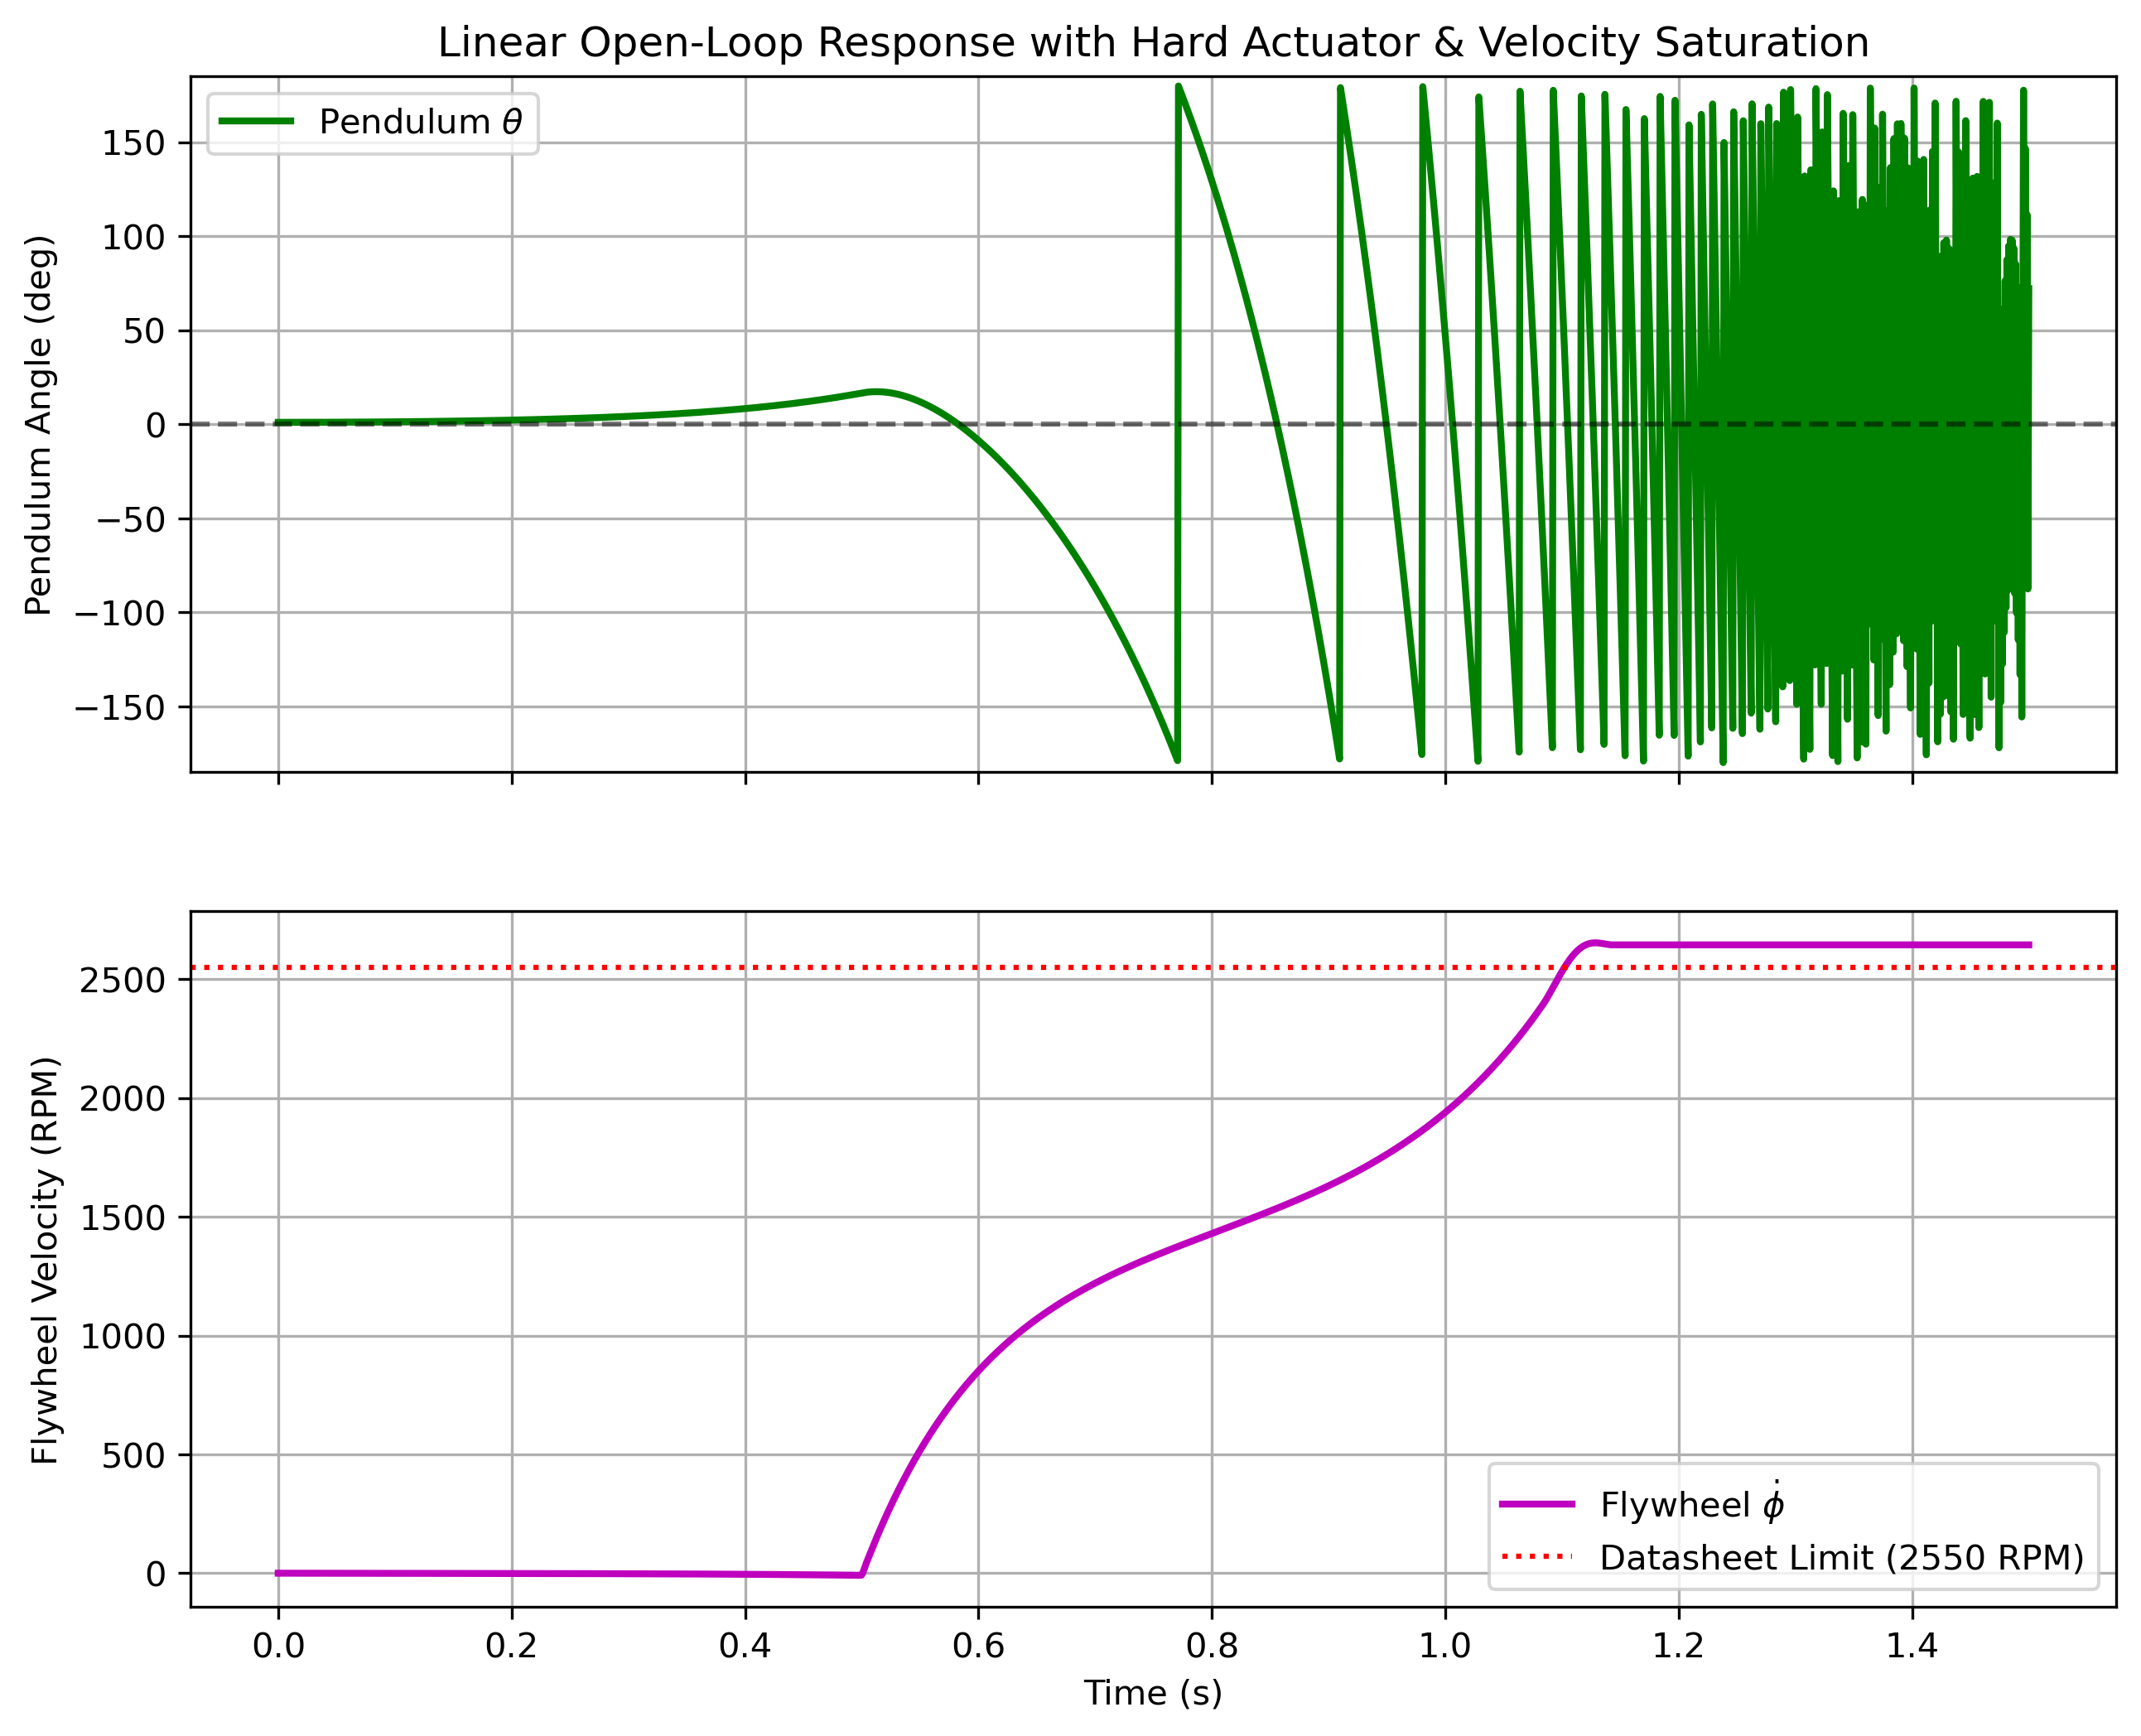
\includegraphics[width=0.75\linewidth]{../outputs/plots/part_a/linear_open_loop_step_response.png}
	\caption{پاسخ پله حلقه باز مدل خطی سیستم پاندول معکوس}
	\label{fig:linear_open_loop_step_response}
\end{figure}

\subsection{پاسخ غیرخطی و رفتار واقعی سیستم}
با اعمال یک پالس یا پله ولتاژ روی مدل غیرخطی کامل (شبیه‌سازی‌شده در فایل‌های \lr{\texttt{02\_open\_loop\_sim.py}} و \lr{\texttt{02\_open\_loop\_nonlinear\_response.py}})، پاندول در اثر گشتاور عکس‌العمل از حالت قائم خارج شده و سقوط می‌کند. موتور با رسیدن به سرعت نامی دیتاشیت متوقف از افزایش سرعت می‌شود (اشباع ذاتی) و پاندول حول زاویه ۱۸۰- درجه (آویزان پایین) دچار نوسانات نامیرا در اثر تزریق متناوب انرژی و اصطکاک ($b_0$) می‌گردد که این پدیده عینی در اشکال زیر مستند شده است.

\begin{figure}[h!]
	\centering
	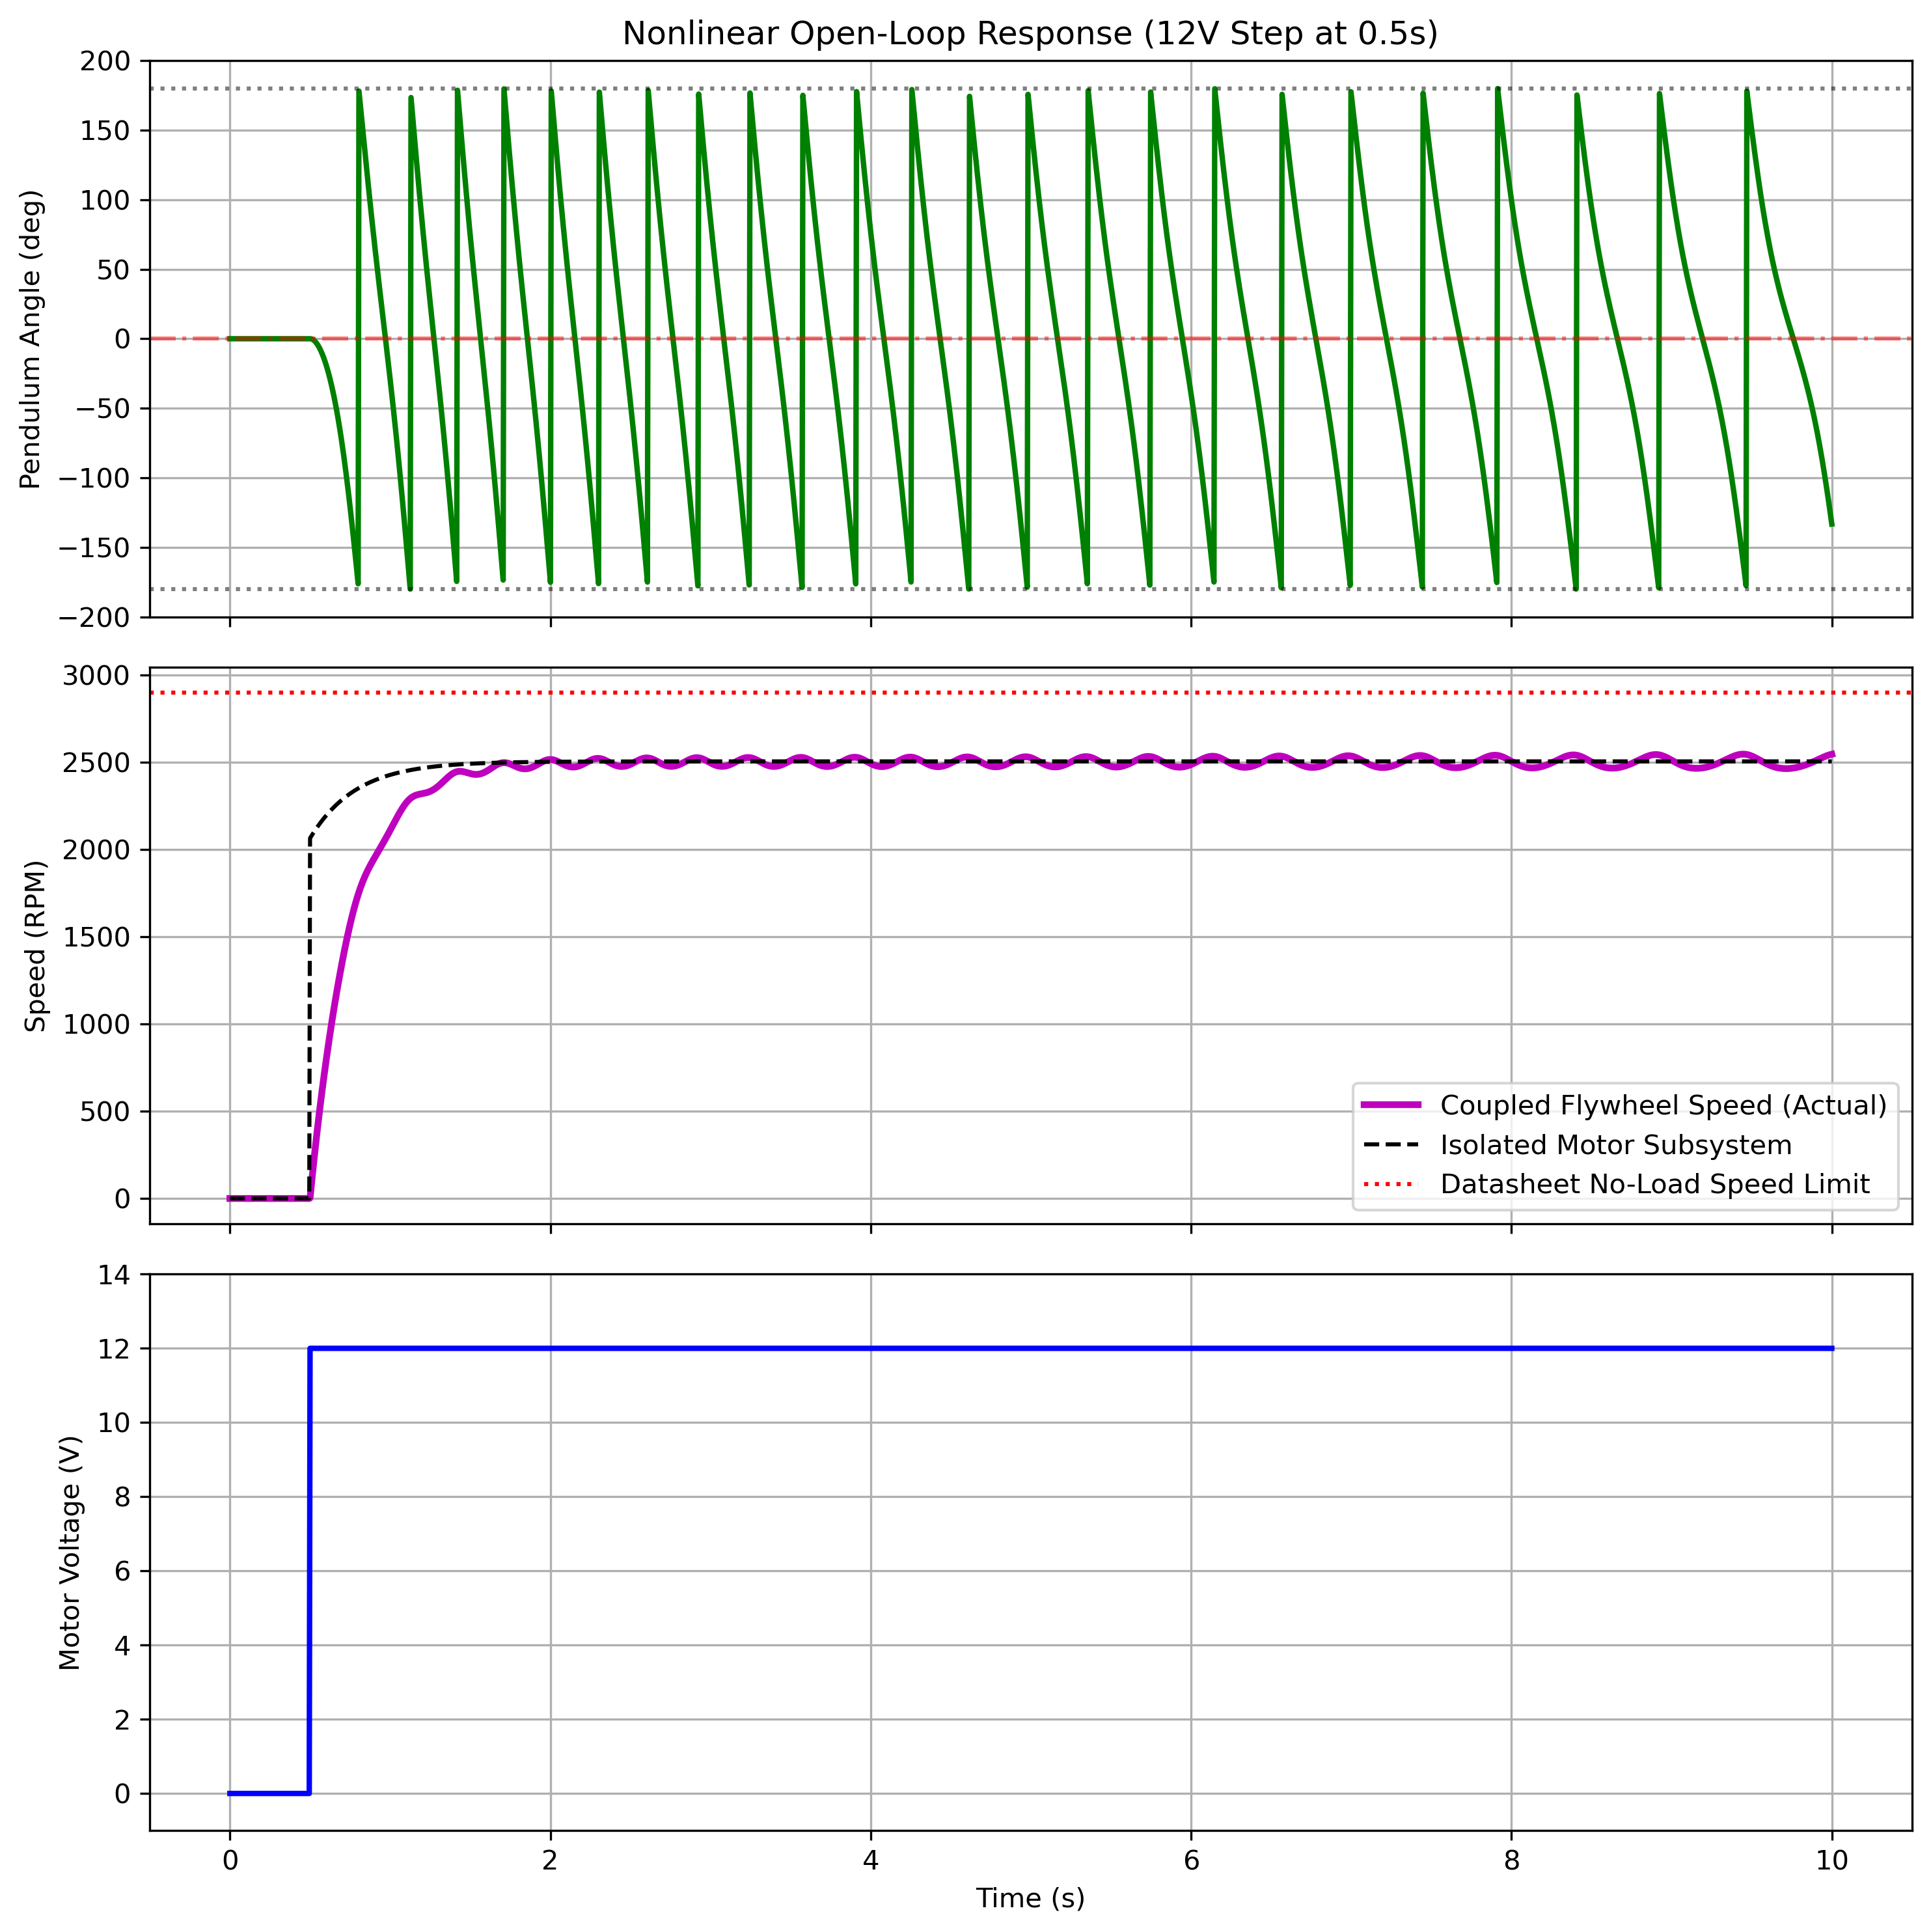
\includegraphics[width=0.75\linewidth]{../outputs/plots/part_a/02_open_loop_nonlinear_response.png}
	\caption{پاسخ غیرخطی حلقه باز به ورودی پله ولتاژ}
	\label{fig:02_open_loop_nonlinear_response}
\end{figure}

\begin{figure}[h!]
	\centering
	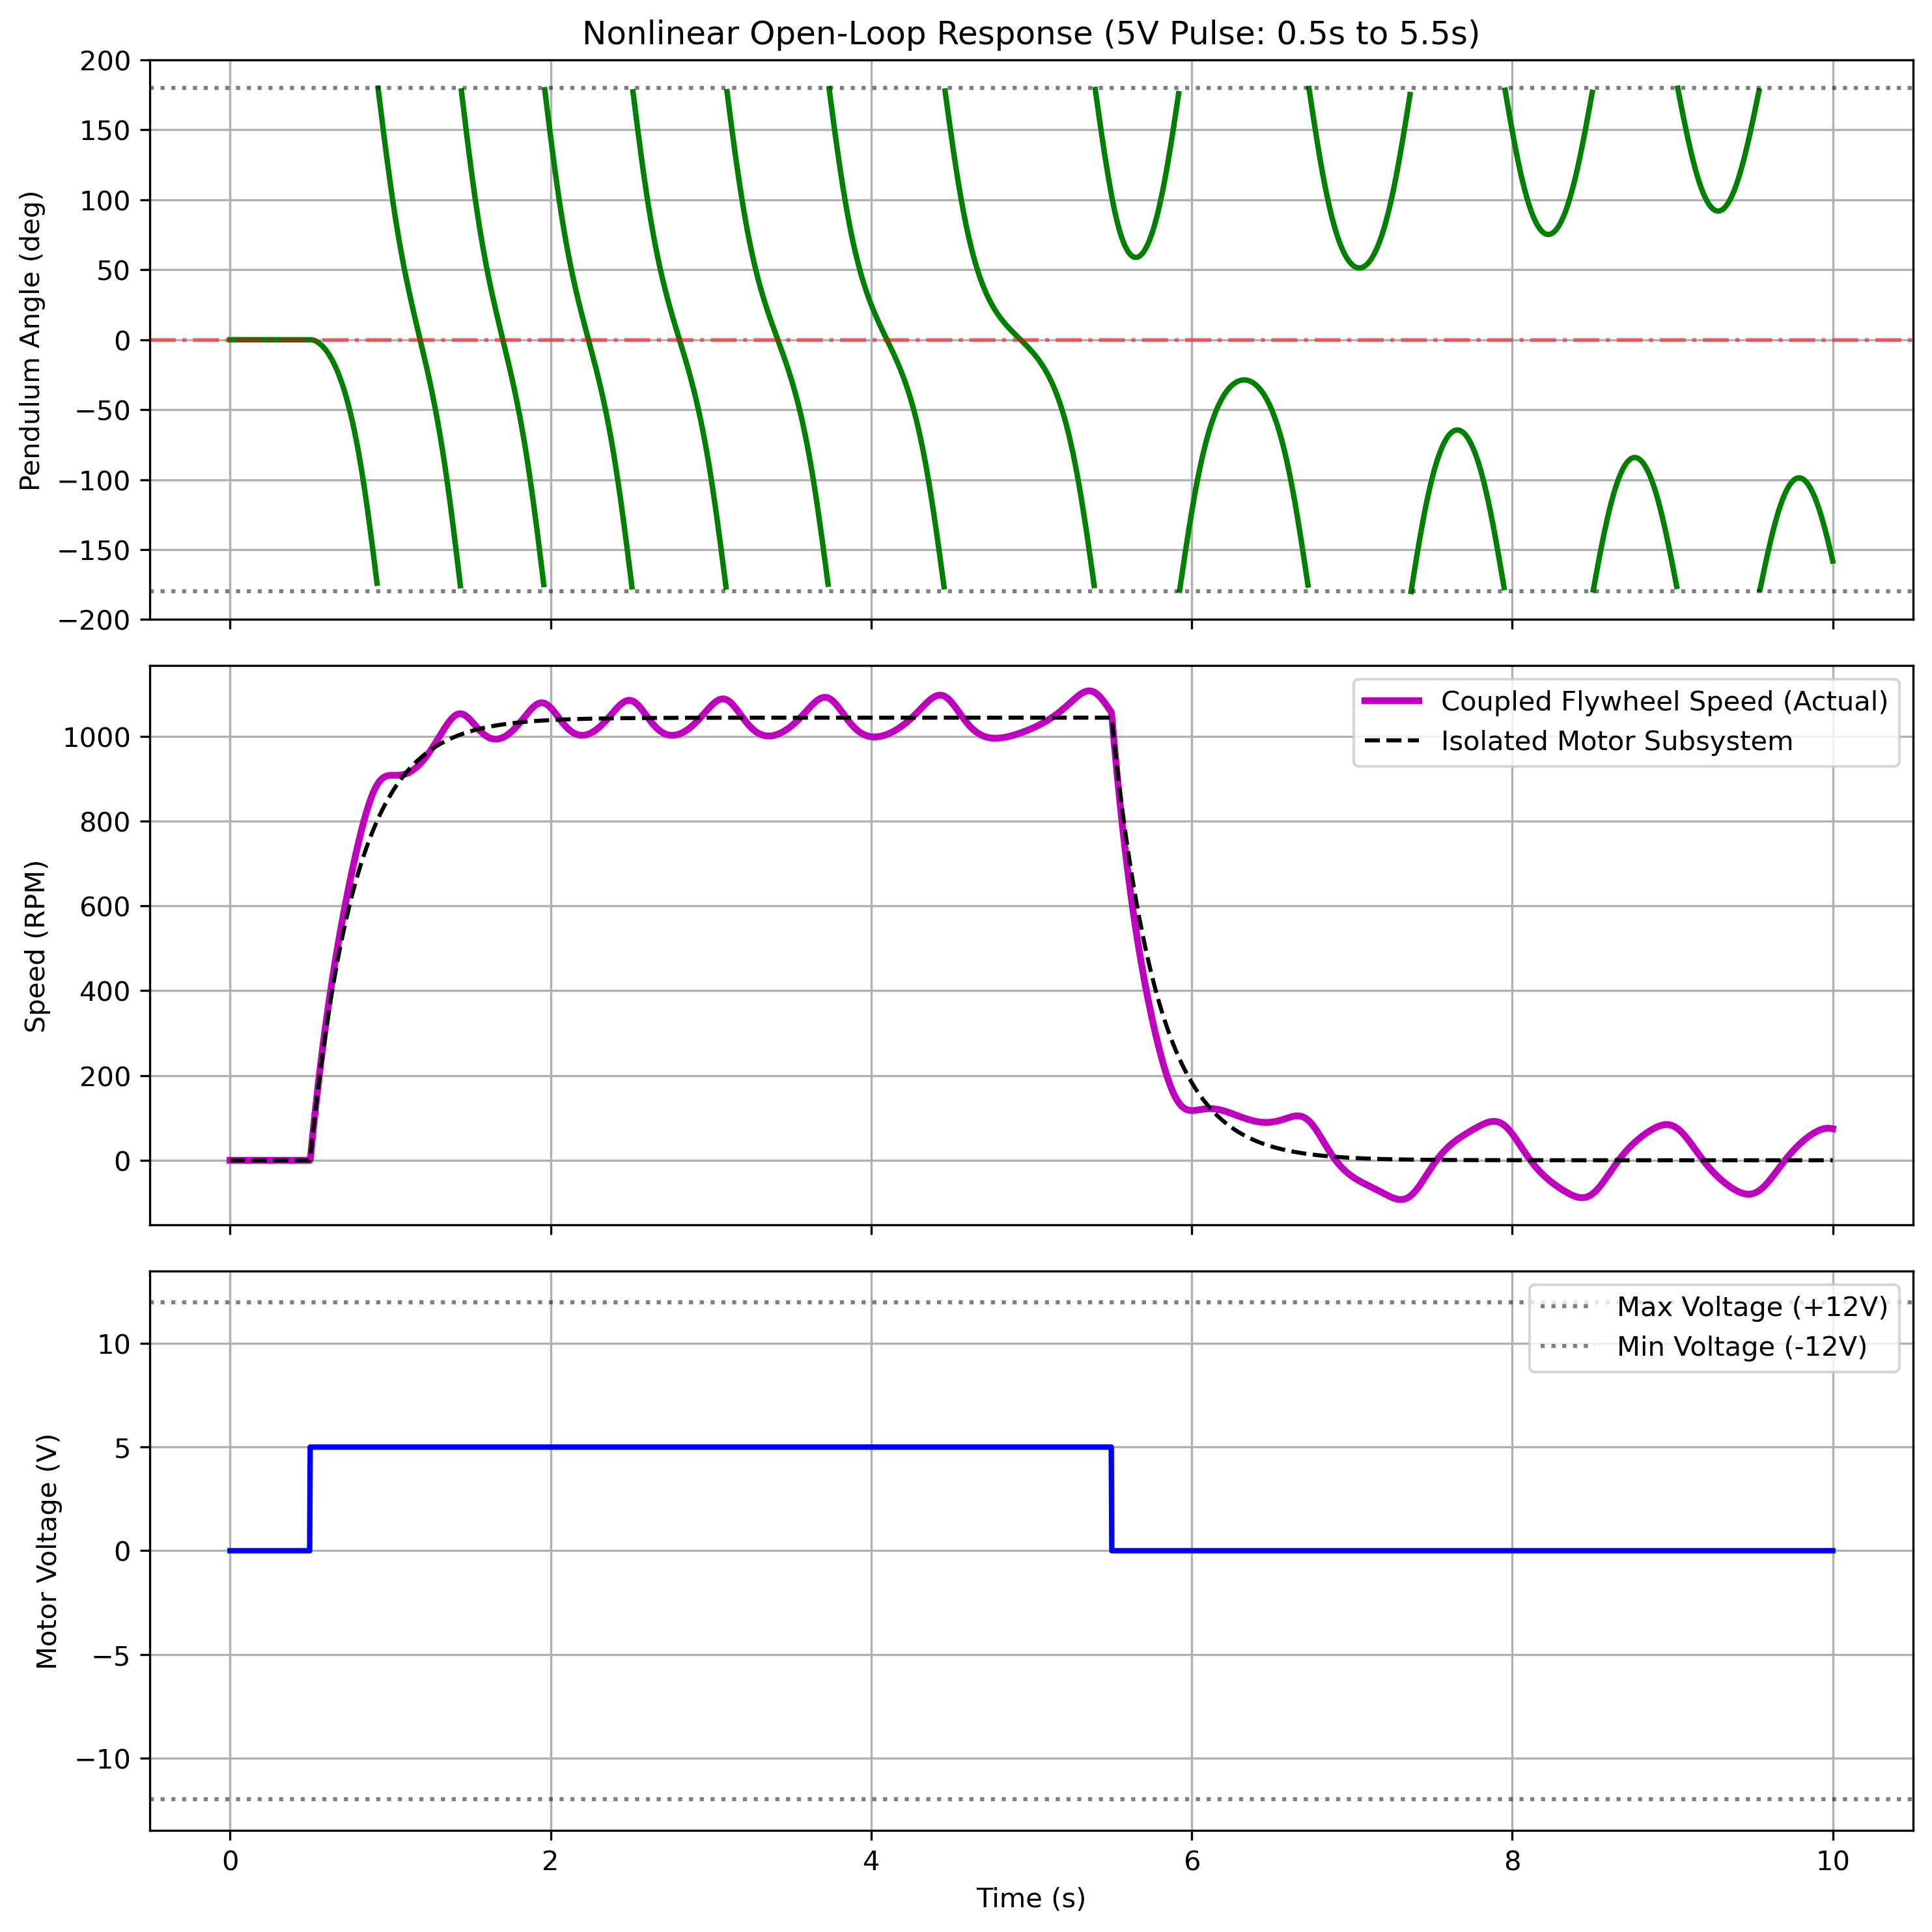
\includegraphics[width=0.75\linewidth]{../outputs/plots/part_a/02_open_loop_nonlinear_pulse.png}
	\caption{پاسخ غیرخطی حلقه باز به ورودی پالس ولتاژ}
	\label{fig:02_open_loop_nonlinear_pulse}
\end{figure}

\section{طراحی کنترل‌کننده \lr{PID} و کشف گلوگاه سیستمی}

\subsection{استراتژی تنظیم ضرایب (\lr{Tuning}) روی مدل غیرخطی}
به جای روش‌های سعی‌وخطای کلاسیک، از الگوریتم بهینه‌سازی بدون مشتق \lr{Nelder-Mead} در فایل \\
\lr{\texttt{03\_closed\_loop\_pid\_sim.py}} \\
برای تنظیم ضرایب \lr{PID} روی شبیه‌ساز غیرخطی استفاده شد. تابع هزینه $J$ شامل خطای تجمعی زاویه، جریمهٔ شدید سقوط ($\theta > 80^\circ$) و جریمهٔ اشباع ولتاژ به همراه نرخ تغییرات ولتاژ (\lr{Slew Rate} = $120 \text{ \lr{V/s}}$) بود. ضرایب نهایی به شرح زیر استخراج شدند:
\[ K_p = 300, \quad K_i = 150, \quad K_d = 0.1 \]

\subsection{توهم پایداری در برابر اغتشاش پله (اصلاحیه تحلیلی)}
در بررسی اولیه شبیه‌سازی کوتاه ۱۵ ثانیه‌ای که نمودار آن در شکل \ref{fig:full_motor_response_dist_0.02} آورده شده است، پاسخ سیستم به اغتشاش پله‌ای $0.02 \text{ \lr{Nm}}$ کاملاً پایدار ارزیابی شد. اما تحلیل عمیق مهندسی ثابت کرد این نتیجه یک \textbf{خطای معرفتی ناشی از محدودیت پنجرهٔ زمان شبیه‌سازی} بوده است.

\begin{figure}[h!]
	\centering
	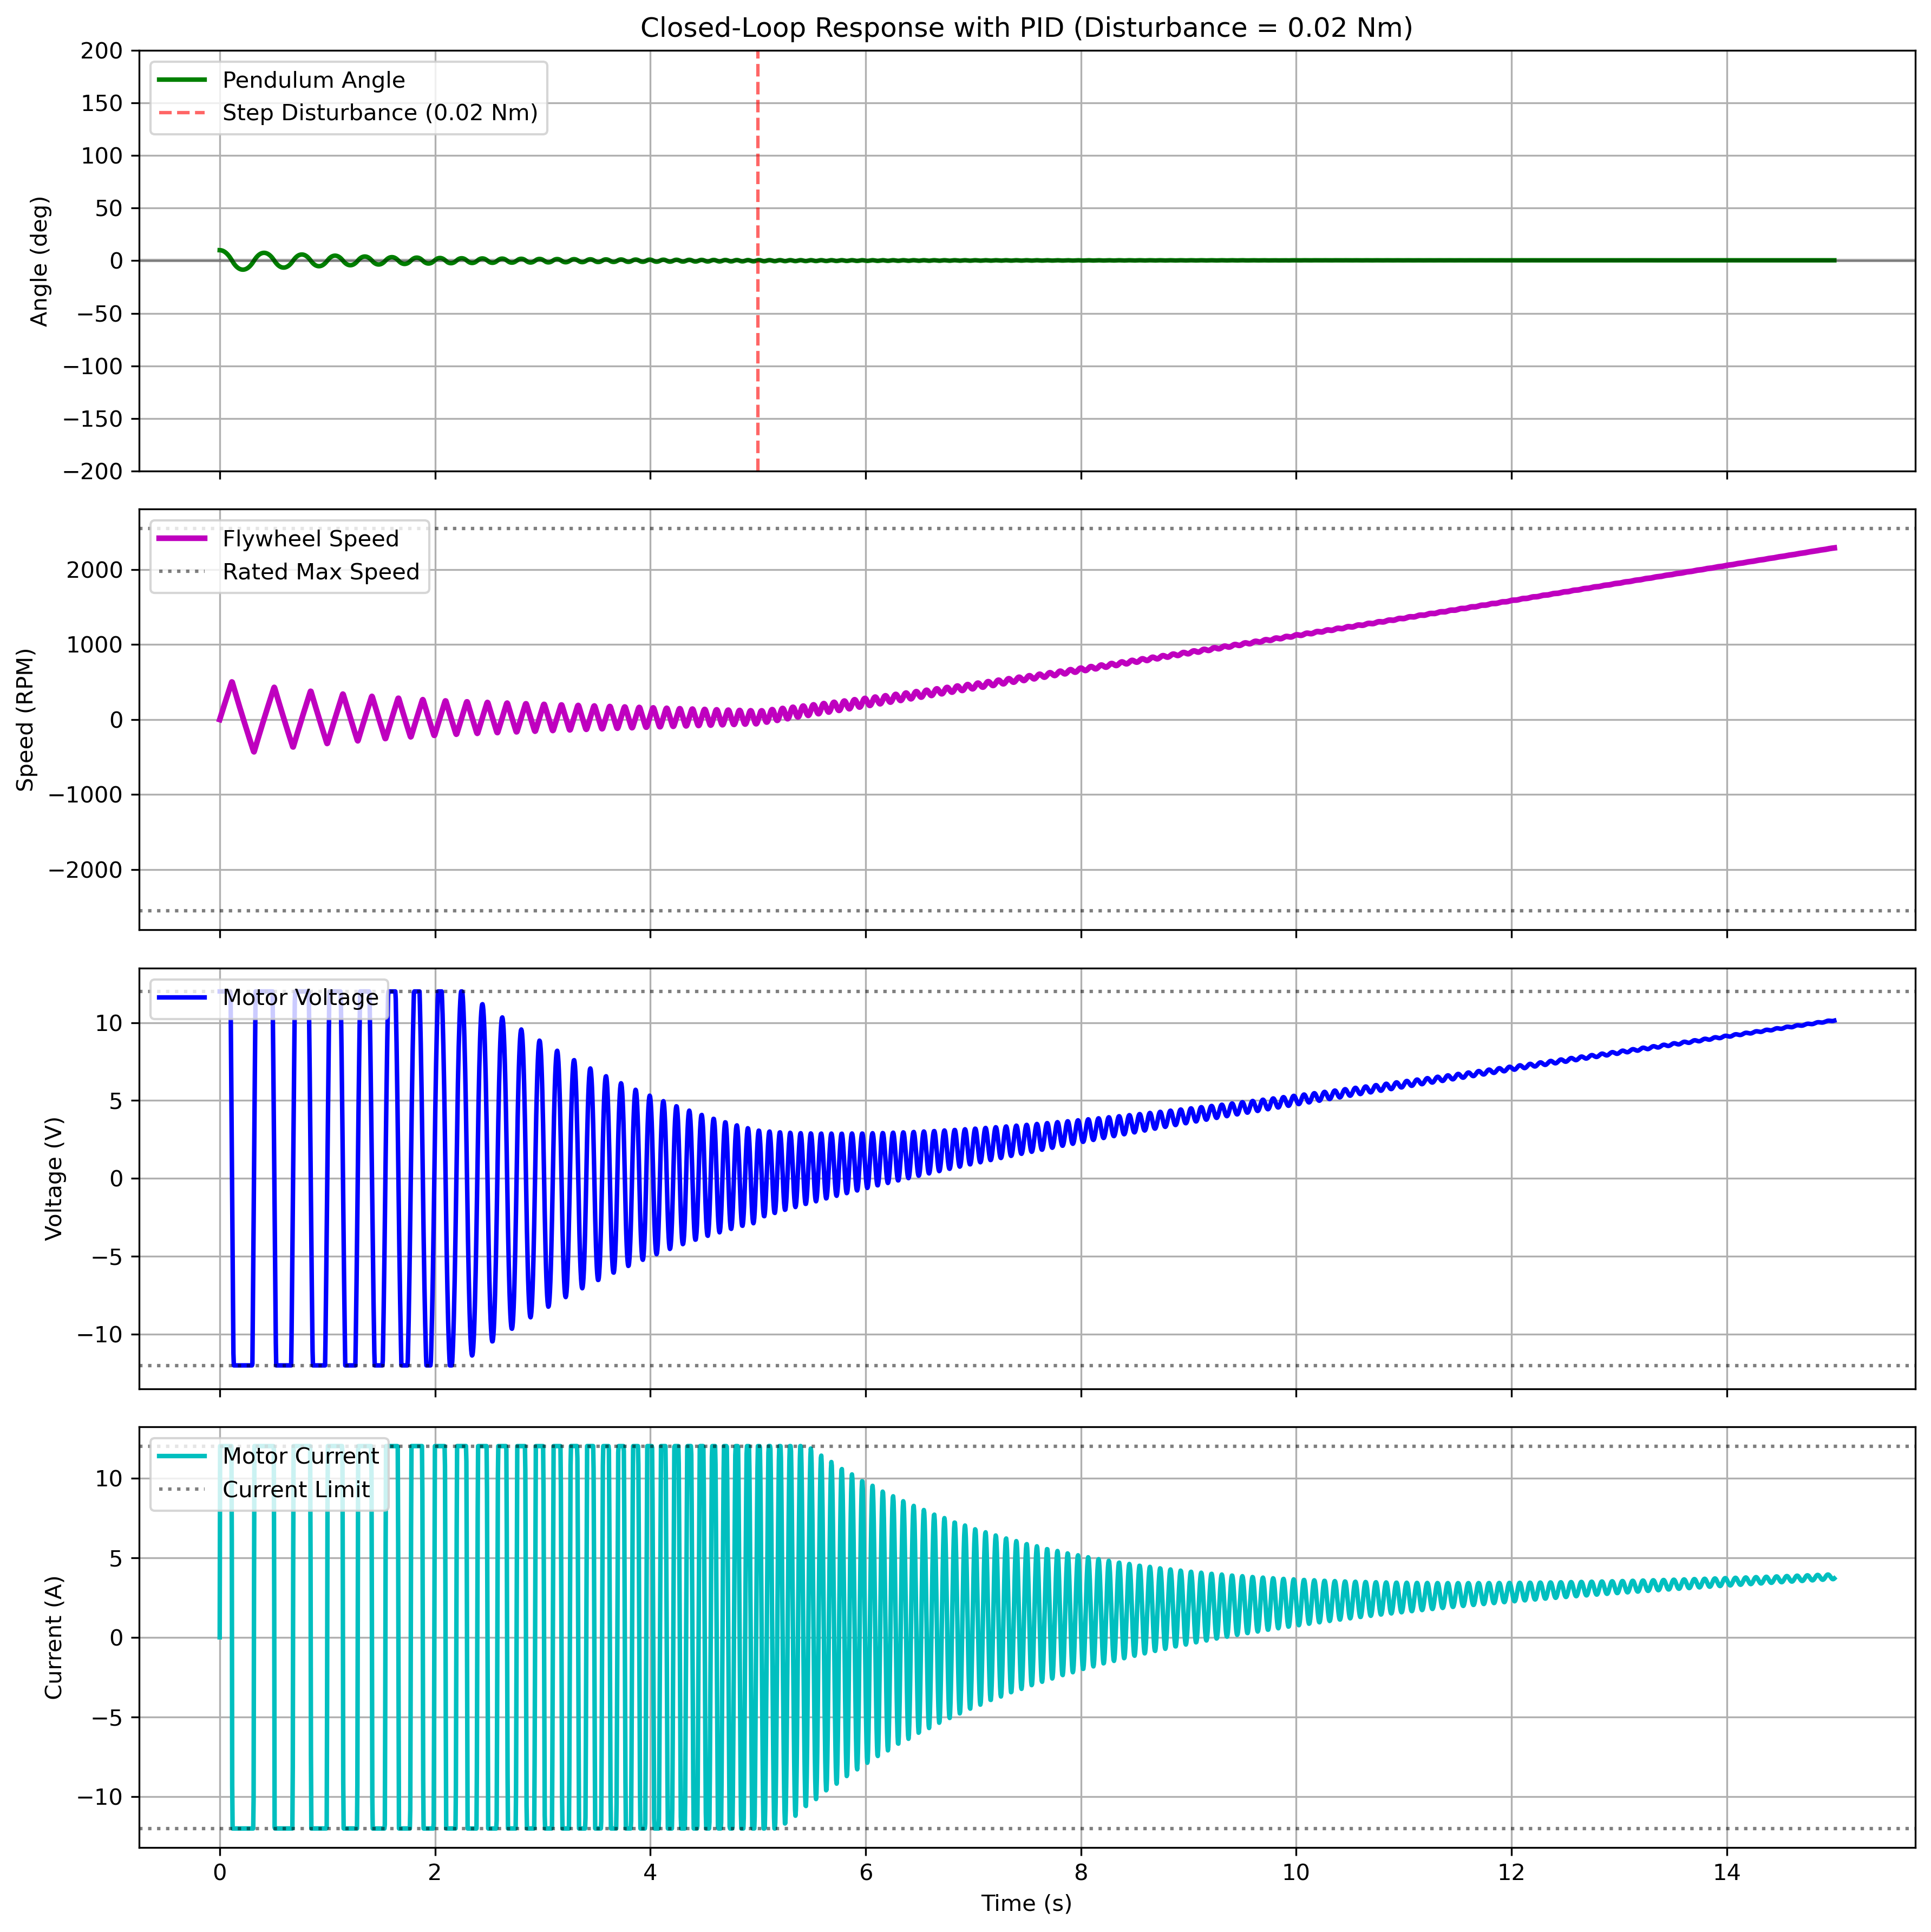
\includegraphics[width=0.75\linewidth]{../outputs/plots/part_a/full_motor_response_dist_0.02.png}
	\caption{پاسخ سیستم تحت کنترلر \lr{PID} به اغتشاش پله‌ای کوچک $0.02 \text{ \lr{Nm}}$ (نمایش پایداری موقت)}
	\label{fig:full_motor_response_dist_0.02}
\end{figure}

\subsection{اثبات تئوریک عدم امکان خنثی‌سازی اغتشاش پله}
سیستم چرخ واکنش در مهندسی کنترل به عنوان یک سیستم \textbf{زیرفعال (\lr{Underactuated})} و \textbf{فاز غیر حداقل (\lr{Non-minimum Phase})} شناخته می‌شود که در فرکانس‌های صفر (حالت ماندگار پاسخ پله) دارای یک قطب در مبدأ در تابع تبدیل گشتاور به سرعت چرخ است. این بدین معناست که سیستم اصلاً توانایی خنثی‌سازی خطای حالت ماندگار اغتشاش پله را بدون واگرایی و فرار سرعت چرخ ندارد.

کنترلر \lr{PID} با افزودن ترم انتگرال‌گیر ($K_i$) تلاش می‌کند خطای حالت ماندگار زاویه میله پاندول ($\theta$) را صفر کند. اما در ادامه به صورت ریاضی اثبات می‌شود که صفر شدن این خطا، لزوماً به قیمت ناپایداری متغیر حالت دوم یعنی سرعت چرخ ($\dot{\phi}$) تمام خواهد شد.

با اعمال تابع پله در ورودی اغتشاش به صورت $T_{dist}(s) = \frac{D}{s}$، طبق قضیه مقدار نهایی (\lr{Final Value Theorem}) نشان داده می‌شود که برای حفظ پایداری زاویه بازو در نقطه تعادل ($\theta \to 0$)، باید گشتاور خروجی موتور در حالت ماندگار دقیقاً برابر با مقدار ثابت اغتشاش خارجی گردد تا اثر گرانش غیرتعادلی خنثی شود ($\tau_m = T_{dist}$). با جاگذاری این مقدار گشتاور در معادله دینامیکی مستقل چرخ هرزگرد داریم:
\[ \dot{\phi}(t) = \frac{1}{J_f} \int_{t_0}^{t} \tau_m \, dt \implies \dot{\phi}(t) = \frac{T_{dist}}{J_f} \cdot t \]
این رابطه ریاضی (که نشان‌دهنده رفتار ریمپ یا همان شیب صعودی خطی در سرعت چرخ است) اثبات می‌کند که فرار سرعت چرخ یک پدیده کاملاً ساختاری و ذاتی فیزیک سیستم است و هیچ ارتباطی به نحوه تنظیم یا بهینه بودن گین‌های کنترل‌کننده \lr{PID} ندارد.

\subsection{مکانیزم مدل‌سازی اشباع سرعت فیزیکی}
در لایه نرم‌افزاری شبیه‌ساز پایتون، برای شبیه‌سازی دقیق فیزیکی موتور و درایور، ساختار منطقی زیر جهت اعمال قیدهای مکانیکی سخت‌افزاری بر روی شتاب‌گیری فلایویل پیاده‌سازی شده است. با رسیدن سرعت زاویه‌ای چرخ به مرز فیزیکی حداکثر سرعت نامی موتور یعنی $\Omega_{max}$ (معادل $2550 \text{ \lr{RPM}}$)، توانایی اعمال گشتاور موتور در جهت سرعت دوران طبق رابطه منطقی زیر به صفر میل می‌کند:
\[ \text{If } |\dot{\phi}| \ge \Omega_{max} \quad \text{and} \quad \text{sgn}(\dot{\phi}) = \text{sgn}(i_a) \implies \tau_{motor} = 0 \]
این مکانیزم به خوبی توضیح می‌دهد که چرا نمودار جریان و ولتاژ پس از برخورد به سقف مکانیکی دچار افت ناگهانی شده و قطع کامل گشتاور ترمیمی سبب واگرایی آنی زاویه آونگ و سقوط آزاد سیستم می‌شود.

\subsection{مشخصات زمانی پاسخ سیستم و کرونولوژی رفتاری}
برای درک جامع رفتار زمانی سیستم بر اساس اجرای شبیه‌سازی ۲۰ ثانیه‌ای تحت اغتشاش پله‌ای ماندگار $0.02 \text{ \lr{Nm}}$، مراحل زمانی رویدادها و واکنش‌های فیزیکی سیستم به تفکیک در جدول \ref{tab:timeline} ثبت شده است.

\begin{table}[h!]
	\centering
	\caption{کرونولوژی رفتاری سیستم تحت اغتشاش $0.02 \text{ \lr{Nm}}$}
	\label{tab:timeline}
	\begin{tabular}{|p{3cm}|p{11cm}|}
		\hline
		\textbf{بازه زمانی (ثانیه)} & \textbf{شرح رفتار فیزیکی و دینامیکی سیستم} \\ \hline
		$t = 0 \text{ to } t = 2$ & میراسازی سریع نوسانات اولیه ناشی از انحراف ۱۰ درجه بازو با مصرف پیک توان در درایور موتور (ولتاژ اشباع $\pm 12 \text{ \lr{V}}$ و پیک جریان آرمیچر). \\ \hline
		$t = 5$ & لحظه دقیق اعمال اغتشاش پله‌ای ناگهانی به بزرگی $0.02 \text{ \lr{Nm}}$ روی میله پاندول. \\ \hline
		$t = 5 \text{ to } t \approx 12.5$ & فاز پایداری ظاهری میله پاندول در نقطه قائم تعادل، هم‌زمان با صعود خطی سرعت چرخ با نرخ شتاب ثابت جهت تامین گشتاور خنثی‌ساز (پدیده واگرایی پنهان تکانه). \\ \hline
		$t \approx 12.5$ & لحظه بحرانی برخورد سرعت زاویه‌ای فلایویل به سقف فیزیکی $2550 \text{ \lr{RPM}}$ و قطع آنی گشتاور تولیدی توسط موتور طبق قید اشباع سرعت. \\ \hline
		$t > 12.5$ & سقوط آزاد پاندول به دلیل عدم تعادل نیروها، واگرایی سریع زاویه بازو و پرش‌های زاویه‌ای روی نمودار به دلیل عبور از مرز دایره‌ای $180^\circ$. \\ \hline
	\end{tabular}
\end{table}

\section{شبیه‌سازی اجسام صلب و موتور رندرینگ سه‌بعدی}
جهت صحه‌گذاری عینی بر رفتار فیزیکی سیستم بدون استفاده از نرم‌افزارهای تجاری سنگین، یک موتور رندرینگ سه‌بعدی اختصاصی با استفاده از ماژول‌های \lr{\texttt{matplotlib.animation}} و کلاس \lr{\texttt{Poly3DCollection}} توسعه یافت. این ابزار هندسه سه بعدی بازو (مکعب مستطیل) و فلایویل (استوانه سه‌بعدی حول محور دوران) را بر اساس زوایای شبیه‌سازی در هر گام ترسیم کرده و انیمیشن نهایی را در قالب فایل‌های ویدیویی \lr{\texttt{full\_system\_multibody\_0.02.mp4}} و \lr{\texttt{inverted\_pendulum\_step\_response.mp4}} ذخیره می‌نماید که برای صحه‌گذاری فیزیکی بسیار کارآمد است.

\section{معماری پیشرفته: ماشین حالت، نوسان‌آوری و مدیریت تکانه}
برای غلبه بر محدودیت‌های تحلیل‌شده در کنترلر \lr{PID}، یک سوپروایزر منطقی (ماشین حالت) مبتنی بر روش‌های کنترل \\
انرژی و فیدبک حالت بهینه در فایل‌های \lr{\texttt{09\_10\_swingup\_lqr\_momentum\_dump.py}} و \lr{\texttt{99\_full\_lifecycle\_35s.py}} طراحی و پیاده‌سازی شد. نمودارهای زمانی این مانور جامع در اشکال بعدی منعکس شده است.

\subsection{فاز اول: سقوط (\lr{Fall State})}
سیستم تحت اغتشاش توسط \lr{PID} کنترل می‌شود. با رسیدن سرعت موتور به مرز اشباع مکانیکی/الکتریکی، سیستم توان جبران را از دست داده و سقوط می‌کند. ماشین حالت با عبور زاویه پاندول از مرز بحرانی $80^\circ$ این شکست را تشخیص داده، ولتاژ موتور را سریعاً صفر می‌کند تا انرژی سیستم توسط اصطکاک طبیعی لولا میرا شود (ناحیه خاکستری در نمودار مدهای کنترلی).

\subsection{فاز دوم: نوسان‌آوری مبتنی بر انرژی (\lr{Swing-up})}
گشتاور موتور به تنهایی قادر به غلبه بر نیروی جاذبه برای بلند کردن مستقیم پاندول از زاویه آویزان $180^\circ$ نیست. راهکار مهندسی، «تزریق کار مکانیکی مثبت» به صورت گام‌به‌گام به سیستم است. کنترل‌کننده نوسان‌آور انرژی‌محور به شکل زیر فرموله و اعمال شد:
\[ V_{cmd} = k \cdot (E_{kin} + E_{pot}) \cdot \dot{\theta} \cdot \cos\theta \]
تطابق علامت سرعت زاویه‌ای ($\dot{\theta}$) با این قانون فرمان، سبب ایجاد نوسان‌های تشدیدی (رزونانس فرکانسی) شده و پالس‌های ولتاژ متناوب در مرز اشباع $\pm 12 \text{\lr{V}}$ تولید می‌کند (ناحیه زرد در نمودار مدهای کنترلی). با این تکنیک، دامنه نوسان به سرعت افزایش یافته تا پاندول وارد ناحیه همسایگی قائم پایدار (\lr{Capture Region}) شود.

\subsection{فاز سوم: تخلیه تکانه و کنترل بهینه (\lr{Momentum Dumping LQR})}
به محض ورود زاویه پاندول به محدوده مجاز نزدیک به قائم (ثانیه ۳۱ شبیه‌سازی)، ماشین حالت کنترل را به رگولاتور بهینه \lr{LQR} واگذار می‌کند (ناحیه سبز در نمودار مدهای کنترلی). جهت ممانعت از انباشت و اشباع سرعت چرخ، به جای کنترلر آبشاری کلاسیک، از فیدبک حالت کامل با ماتریس جریمه زیر استفاده شد:
\[ Q = \text{diag}([2500, 100, 0.5]) \]
این ساختار علاوه بر انحراف پاندول، بر سرعت زاویه‌ای چرخ نیز جریمه اعمال می‌کند.

\textbf{تحلیل دینامیکی مانور تخلیه تکانه:}
الگوریتم \lr{LQR} متوجه سرعت بسیار بالای چرخ (ناشی از تزریق انرژی در فاز نوسان‌آوری) می‌شود. برای ترمز کردن چرخ بدون سقوط پاندول، کنترل‌کننده به طور هوشمندانه پاندول را مقدار کوچکی از حالت کاملاً قائم منحرف می‌کند. این انحراف عامدانه باعث ایجاد یک گشتاور گرانشی پسماند در جهت خلاف دوران چرخ شده و انرژی دورانی فلایویل را در طول ۱۵ ثانیه به‌طور کامل بدون از دست رفتن تعادل روی صفر رگوله می‌کند.

\begin{figure}[h!]
	\centering
	
\includegraphics[width=0.75\linewidth]{../outputs/plots/part_a/05_modes_disturbance_plot.png}
	\caption{نمودار تغییرات مدهای ماشین حالت در چرخه حیات کامل سیستم}
	\label{fig:05_modes_disturbance_plot}
\end{figure}

\begin{figure}[h!]
	\centering
	
\includegraphics[width=0.75\linewidth]{../outputs/plots/part_a/05_angle_plot.png}
	\caption{پاسخ زمانی زاویه پاندول در طی فازهای مختلف کاری}
	\label{fig:05_angle_plot}
\end{figure}

\begin{figure}[h!]
	\centering
	
\includegraphics[width=0.75\linewidth]{../outputs/plots/part_a/05_rpm_plot.png}
	\caption{سرعت دوران چرخ عکس‌العملی بر حسب دور بر دقیقه و فاز تخلیه تکانه}
	\label{fig:05_rpm_plot}
\end{figure}

\begin{figure}[h!]
	\centering
	
\includegraphics[width=0.75\linewidth]{../outputs/plots/part_a/05_voltage_plot.png}
	\caption{سیگنال ولتاژ اعمالی به موتور آرمیچر در چرخه کامل عملیاتی}
	\label{fig:05_voltage_plot}
\end{figure}

\section{راه‌کارهای فرار از گلوگاه اشباع}
یک تحلیل مهندسی کامل در سطح پروژه‌های پیشرفته صنعتی نباید صرفاً به نمایش فروپاشی و سقوط سیستم ختم شود. بر اساس یافته‌های این شبیه‌سازی، سه استراتژی مدرن برای جلوگیری از اشباع تکانه و پایداری درازمدت سیستم تحت اغتشاش‌های ثابت پیشنهاد می‌شود:

\begin{enumerate}
	\item \textbf{مکانیزم تخلیه فعال تکانه زاویه‌ای (\lr{Active Momentum Desaturation}):} اعمال گشتاورهای معکوس و ضربه‌ای کوچک به چرخ هرزگرد در جهت‌هایی از مسیر نوسانی پاندول که بازو در حال بازگشت طبیعی به سمت مرکز است، به گونه‌ای که برآیند اغتشاشات به سرعت چرخ آسیب نزند.
	\item \textbf{کنترل زاویه متمایل به کار (\lr{Lean Angle Control}):} اجازه دادن به پاندول برای ایستادن در یک زاویه غیرصفر بسیار کوچک ماندگار ($\theta_{steady} \neq 0$). در این استراتژی، گشتاور گرانشی ناشی از وزن میله پاندول، اثر گشتاور اغتشاش ثابت خارجی را در حالت ماندگار کاملاً خنثی کرده و نیاز به شتاب‌گیری مداوم چرخ واکنش و صرف گشتاور مداوم از سوی موتور را به صفر می‌رساند.
	\item \textbf{کنترل پیش‌بین مبتنی بر مدل (\lr{MPC}):} استفاده از ساختارهای بهینه‌سازی مقید بر روی متغیرهای حالت به صورت برخط، به گونه‌ای که سرعت زاویه‌ای چرخ به عنوان یک قید نامساوی سخت‌افزاری در مسئله بهینه‌سازی تعریف شده و پیش از رسیدن سرعت به آستانه اشباع، رفتار کنترلی تغییر فاز دهد.
\end{enumerate}

\section{تحلیل مهاجرت نرم‌افزاری (\lr{Python vs. Simulink})}
انتقال صد درصدی مدل‌سازی و کنترل از محیط متلب/سیمولینک به بستر زبان برنامه‌نویسی پایتون پیامدهای مهندسی شفافی به همراه داشت که ارزیابی موازنه مابین دستاوردها و هزینه‌های آن به شرح زیر تبیین می‌گردد:

\begin{itemize}
	\item \textbf{دستاوردهای فنی و ساختاری:} این مهاجرت امکان دسترسی سطح پایین به حل‌گر عددی معادلات دیفرانسیل غیرخطی (\lr{RK45} در کلاس \lr{\texttt{scipy.integrate.solve\_ivp}}) را فراهم نمود که دستکاری بردارهای وضعیت و جلوگیری از ناپیوستگی در لحظه اشباع سرعت موتور را تسهیل کرد. همچنین عدم نیاز به لایسنس‌های تجاری متلب، امکان اجرای شبیه‌سازی به صورت بدون‌واسطه‌گرافیکی (\lr{Headless}) روی سرورهای پردازشی لینوکس اوبونتو و قابلیت نسخه‌بندی خط‌به‌خط ساختار یافته کدها با ابزار \lr{Git} از دستاوردهای بارز این رویکرد به شمار می‌روند.
	\item \textbf{قابلیت‌های از دست‌رفته و هزینه‌ها:} در مقابل، این مهاجرت به معنای از دست دادن محیط بصری و بسیار کارآمد ردیابی سیگنال‌ها (\lr{Visual Signal Tracing}) در سیمولینک بود. پیاده‌سازی گسسته‌زمان توابع تشخیص عبور از صفر (\lr{Zero-crossing detection}) برای سوئیچینگ مدهای ماشین حالت باید از نو به صورت دستی کدنویسی می‌شد. مضاف بر این، فقدان جعبه‌ابزار \lr{Simscape} باعث شد که محاسبات فیزیکی و رندرینگ انیمیشن سه‌بعدی کاملاً با نوشتن فرمول‌های هندسی و ریاضی محض پیاده‌سازی شود که سربار توسعه نرم‌افزار را به شدت بالا برد.
\end{itemize}

\section{نتیجه‌گیری نهایی}
توسعه شبیه‌سازی چرخه حیات کامل سیستم \lr{RWIP} نشان داد که محدودیت اصلی پایداری این سیستم‌ها، گشتاور نامی اکچویتور نیست، بلکه «ظرفیت جذب تکانه زاویه‌ای» فلایویل است. استفاده از کنترلرهای خطی خطایاب کلاسیک مانند \lr{PID} در مواجهه با اغتشاشات مداوم به شکست حتمی می‌انجامد. جایگزینی این استراتژی با ماشین حالت هیبرید مجهز به کنترل انرژی غیرخطی و تنظیم چندمتغیره \lr{LQR} به عنوان یک راهکار صریح علمی، پایداری مجانبی سراسری (\lr{Global Asymptotic Stability}) را با موفقیت تضمین کرد.
\chapter{تحلیل و شبیه‌سازی سیستم دورعملیات دوطرفه (\lr{Bilateral Teleoperation}) با تاخیر زمانی متغیر}

\section{چکیده و ساختار کلی سیستم}
این بخش به بررسی، مدل‌سازی دینامیکی مبنایی، توسعه الگوریتم‌های شبیه‌سازی عددی و تحلیل جامع رفتاری یک سیستم دورعملیات (\lr{Teleoperation}) دوطرفه متشکل از دو ربات بازویی دو درجه آزادی مفصلی صفحه‌ای (\lr{2-DOF RR Planar Manipulator}) می‌پردازد. معماری کلی سیستم بر پایه تعامل مستقیم اپراتور انسانی با ربات محلی (\lr{Local/Master}) بنا شده است؛ اپراتور با اعمال گشتاور فیزیکی پله‌ای، موقعیت بازو را تغییر داده و فرمان حرکتی را تولید می‌کند. این اطلاعات از طریق یک کانال ارتباطی با تاخیر متغیر به ربات راه دور (\lr{Remote/Slave}) مخابره می‌شود تا ربات مقصد، حرکت ربات مبدا را ردیابی کند. در این معماری خاص، هیچ بازخورد نیرویی از ربات راه دور به ربات محلی اعمال نمی‌شود و تنها هدف، دنبال‌کردن موقعیت ربات محلی توسط ربات راه‌دور است. چالش اصلی و گلوگاه پایداری در این معماری، وجود تاخیرهای ارتباطی متغیر با زمان در کانال رفت و برگشت داده است که بر اساس تئوری سیستم‌های ابعاد نامحدود، فاز منفی شدیدی به حلقه پسخورد تزریق می‌کند. به منظور مهار این چالش، ساختار کنترلی صلب بر پایه فیدبک تناسبی-میرایی (\lr{PD}) تنظیم شده و شبیه‌سازی عددی آن در بستر زبان پایتون با طراحی حل‌گر تخصصی پیاده‌سازی شده است.

\section{مدل‌سازی دینامیکی ربات‌های ۲-درجه آزادی صفحه‌ای}
استخراج معادلات حاکم بر مکانیک ربات‌های محلی و راه دور بر اساس فرمول‌بندی اویلر-لاگرانژ و با فرض صلب بودن پیوندها (\lr{Rigid Links}) صورت پذیرفته است. تابع لاگرانژین سیستم به صورت تفاضل انرژی جنبشی کل ($K$) و انرژی پتانسیل کل ($P$) به فرم $L = K - P$ توصیف می‌شود. با جایگذاری این تابع در معادله دیفرانسیل لاگرانژ، معادله حرکت غیرخطی و جفت‌شده برای هر دو ربات به فرم استاندارد ماتریسی زیر استخراج می‌گردد:
\[ M(q)\ddot{q} + C(q, \dot{q})\dot{q} + G(q) = \tau_{ext} \pm \tau_{ctrl} \]
(علامت $\pm$ بسته به جهت اعمال گشتاور در هر ربات متفاوت است). در این فرمول‌بندی، $q = [q_1, q_2]^T$ بردار مختصات تعمیم‌یافته مفاصل دورانی ربات، $\dot{q}$ بردار سرعت زاویه‌ای مفاصل و $\ddot{q}$ بردار شتاب زاویه‌ای مفاصل است. ماتریس‌های دینامیکی برای این بازوی دو درجه آزادی صفحه‌ای به صورت صریح به شرح زیر تعریف می‌شوند:

\textbf{ماتریس اینرسی جرم کل سیستم $M(q)$:}
این ماتریس متقارن و مثبت معین بوده و توزیع جرم و اینرسی لینک‌ها را در فضای مفصلی نشان می‌دهد:
\[ M(q) = \begin{bmatrix} \alpha + 2\beta \cos(q_2) & \delta + \beta \cos(q_2) \\ \delta + \beta \cos(q_2) & \delta \end{bmatrix} \]

\textbf{ماتریس کوریولیس و گریز از مرکز $C(q, \dot{q})$:}
این ماتریس اثرات نیروهای غیرخطی ناشی از جفت‌شدگی سرعت مفاصل را فرمول‌بندی می‌کند:
\[ C(q, \dot{q}) = \begin{bmatrix} -2\beta \sin(q_2)\dot{q}_2 & -\beta \sin(q_2)\dot{q}_2 \\ \beta \sin(q_2)\dot{q}_1 & 0 \end{bmatrix} \]

\textbf{بردار گرانش فیزیکی $G(q)$:}
این بردار گشتاورهای ناشی از شتاب ثقل وارد بر مرکز جرم لینک‌ها را تعیین می‌کند:
\[ G(q) = \begin{bmatrix} \frac{1}{l_2} g \delta \cos(q_1+q_2) + \frac{1}{l_1} g (\alpha - \delta) \cos(q_1) \\ \frac{1}{l_2} g \delta \cos(q_1+q_2) \end{bmatrix} \]
پارامترهای ساختاری ثابت شامل $\alpha$، $\beta$ و $\delta$ توابعی مستقیم از جرم لینک‌ها و طول پیوندها هستند.

\section{مشخصات عددی سناریوی شبیه‌سازی و مشخصات ربات‌ها}
به منظور ارزیابی دقیق، پارامترهای ساختاری بازوها و مفاصل به همراه ضرایب تنظیم‌شده کنترل‌کننده تناسبی-میرایی (\lr{PD}) در قالب جدول \ref{tab:teleop_params} کالیبره شده‌اند.

\begin{table}[h!]
	\centering
	\caption{پارامترهای هندسی، فیزیکی و بهره‌های کنترلی سیستم دورعملیات}
	\label{tab:teleop_params}
	\begin{tabular}{|l|l|l|}
		\hline
		\textbf{پارامتر} & \textbf{ربات محلی (\lr{Local})} & \textbf{ربات راه دور (\lr{Remote})} \\ \hline
		طول لینک اول ($l_1$) & $0.38 \text{ \lr{m}}$ & $0.38 \text{ \lr{m}}$ \\ \hline
		طول لینک دوم ($l_2$) & $0.38 \text{ \lr{m}}$ & $0.38 \text{ \lr{m}}$ \\ \hline
		جرم لینک اول ($m_1$) & $3.9473 \text{ \lr{kg}}$ & $3.2409 \text{ \lr{kg}}$ \\ \hline
		جرم لینک دوم ($m_2$) & $0.6232 \text{ \lr{kg}}$ & $0.3185 \text{ \lr{kg}}$ \\ \hline
		بهره تناسبی ($K$) & $K_l = [20.0, \ 20.0]^T$ & $K_r = [20.0, \ 20.0]^T$ \\ \hline
		بهره میرایی ($B$) & $B_l = [5.0, \ 5.0]^T$ & $B_r = [5.0, \ 5.0]^T$ \\ \hline
	\end{tabular}
\end{table}

\subsection{فرمول‌بندی سیگنال اغتشاش و ورودی اپراتور انسانی}
تحریک سیستم توسط اپراتور انسانی از طریق اعمال گشتاورهای بیرونی زمان‌بندی‌شده بر روی مفاصل بازوی محلی صورت می‌پذیرد. این ورودی به صورت توابع پله‌ای متوالی متغیر در بازه زمانی شبیه‌سازی ۳۵ ثانیه‌ای به صورت ریاضی زیر فرموله شده است:
\[ \tau_{h1}(t) = \begin{cases} 0 & 0 \le t < 5 \\ 10 & 5 \le t < 15 \\ 0 & 15 \le t < 25 \\ 5 & 25 \le t < 35 \end{cases} \quad , \quad \tau_{h2}(t) = \begin{cases} 0 & 0 \le t < 5 \\ 15 & 5 \le t < 15 \\ 20 & 15 \le t < 25 \\ 10 & 25 \le t < 35 \end{cases} \]
در این سناریو، فرض بر این است که ربات راه دور در محیطی آزاد حرکت کرده و با موانع فیزیکی برخورد نمی‌کند؛ از این رو، گشتاور اغتشاش خارجی سمت مقصد صفر لحاظ شده است ($\tau_{ext\_remote} = [0, 0]^T$).

\section{تبدیل معادلات دینامیکی به فرم فضای حالت جهت حل عددی}
الگوریتم‌های حل عددی گام‌به‌گام مانند متد رونگه-کوتا مرتبه چهار (\lr{RK4}) تنها بر روی معادلات دیفرانسیل مرتبه اول عمل می‌کنند. از این رو، شکستن معادلات حرکت به فرم فضای حالت مرتبه اول صریح الزامی است.

با تعریف بردار وضعیت ربات محلی به صورت $x_l = [q_l^T, \dot{q}_l^T]^T$، مشتق زمانی بردار حالت با ایزوله‌سازی شتاب مفاصل به فرم زیر استخراج می‌شود:
\[ \dot{x}_l = \begin{bmatrix} \dot{q}_l \\ \ddot{q}_l \end{bmatrix} = \begin{bmatrix} \dot{q}_l \\ M_l^{-1}(q_l) \left( \tau_h - \tau_l^{ctrl} - C_l(q_l, \dot{q}_l)\dot{q}_l - G_l(q_l) \right) \end{bmatrix} \]
به طریق مشابه، بردار وضعیت برای ربات راه دور به شکل زیر بازنویسی می‌گردد:
\[ \dot{x}_r = \begin{bmatrix} \dot{q}_r \\ \ddot{q}_r \end{bmatrix} = \begin{bmatrix} \dot{q}_r \\ M_r^{-1}(q_r) \left( \tau_r^{ctrl} - C_r(q_r, \dot{q}_r)\dot{q}_r - G_r(q_r) \right) \end{bmatrix} \]
این دو سیستم فضای حالت بزرگ، از طریق سیگنال‌های کنترلی تاخیریافته شبکه به یکدیگر جفت می‌شوند.

\section{ساختار کنترلی و تاخیر ارتباطی متغیر با زمان}
شبکه ارتباطی دیجیتال میان دو ایستگاه، دارای تاخیرهای متغیر با زمان سینوسی فرکانس بالا در مسیرهای رفت و برگشت داده است. این پروفیل‌های تاخیری به صورت زیر مدل‌سازی شده‌اند:
\[ T_l(t) = 0.2 + 0.1\sin(5t) + 0.05\sin(2.5t) \]
\[ T_r(t) = 0.2 + 0.1\sin(2.5t) + 0.05\sin(5t) \]
تاخیر $T_r(t)$ معرف مدت زمان انتقال داده‌های موقعیت از محلی به راه‌دور و $T_l(t)$ نشان‌دهنده مدت زمان بازگشت سیگنال موقعیت از راه‌دور به محلی است. به منظور پایدارسازی سیستم، قوانین کنترلی فیدبک تناسبی-میرایی (\lr{PD}) با \textbf{تأکید بر علامت منفی موجود در معادله دینامیک سمت لوکال} به شکل زیر پیاده‌سازی شدند:

\[ \tau_l^{ctrl} = K_l \left(q_l(t) - q_r(t - T_l(t))\right) + B_l \dot{q}_l(t) \]
\[ \tau_r^{ctrl} = K_r \left(q_l(t - T_r(t)) - q_r(t)\right) - B_r \dot{q}_r(t) \]

نکته بسیار مهم در شبیه‌سازی عددی این است که گشتاور محاسباتی $\tau_l^{ctrl}$، طبق معادله دینامیک لاگرانژ، با علامت منفی به عنوان ورودی به دینامیک ربات محلی اعمال می‌شود (یعنی $-\tau_l^{ctrl}$). این ساختار فیدبک منفی، تضمین می‌کند که ترم $K_l$ یک نیروی بازگرداننده برای ربات محلی ایجاد کرده و ترم میرایی $+B_l\dot{q}_l$ در واقعیت به یک ترم استهلاک انرژی تبدیل می‌شود. ترم‌های میرایی صریح در سمت راه‌دور (شامل $-B_r\dot{q}_r$) نیز وظیفه خروج انرژی و استهلاک نوسانات ناشی از تاخیر شبکه را بر عهده دارند.

\section{تحلیل و ارزیابی جامع نتایج شبیه‌سازی}
پاسخ دینامیکی کل سیستم حلقه بسته در بازه ۳۵ ثانیه‌ای شبیه‌سازی اجرا شده و خروجی‌ها در قالب ۴ نمودار تحلیل می‌شوند.

\subsection{تحلیل عملکرد ردیابی موقعیت مفصل اول}
نمودار خروجی عملکرد ردیابی مفصل اول در شکل \ref{fig:01_Position_Tracking_Performance_Joint_1} نمایش داده شده است.

\begin{figure}[h!]
	\centering
	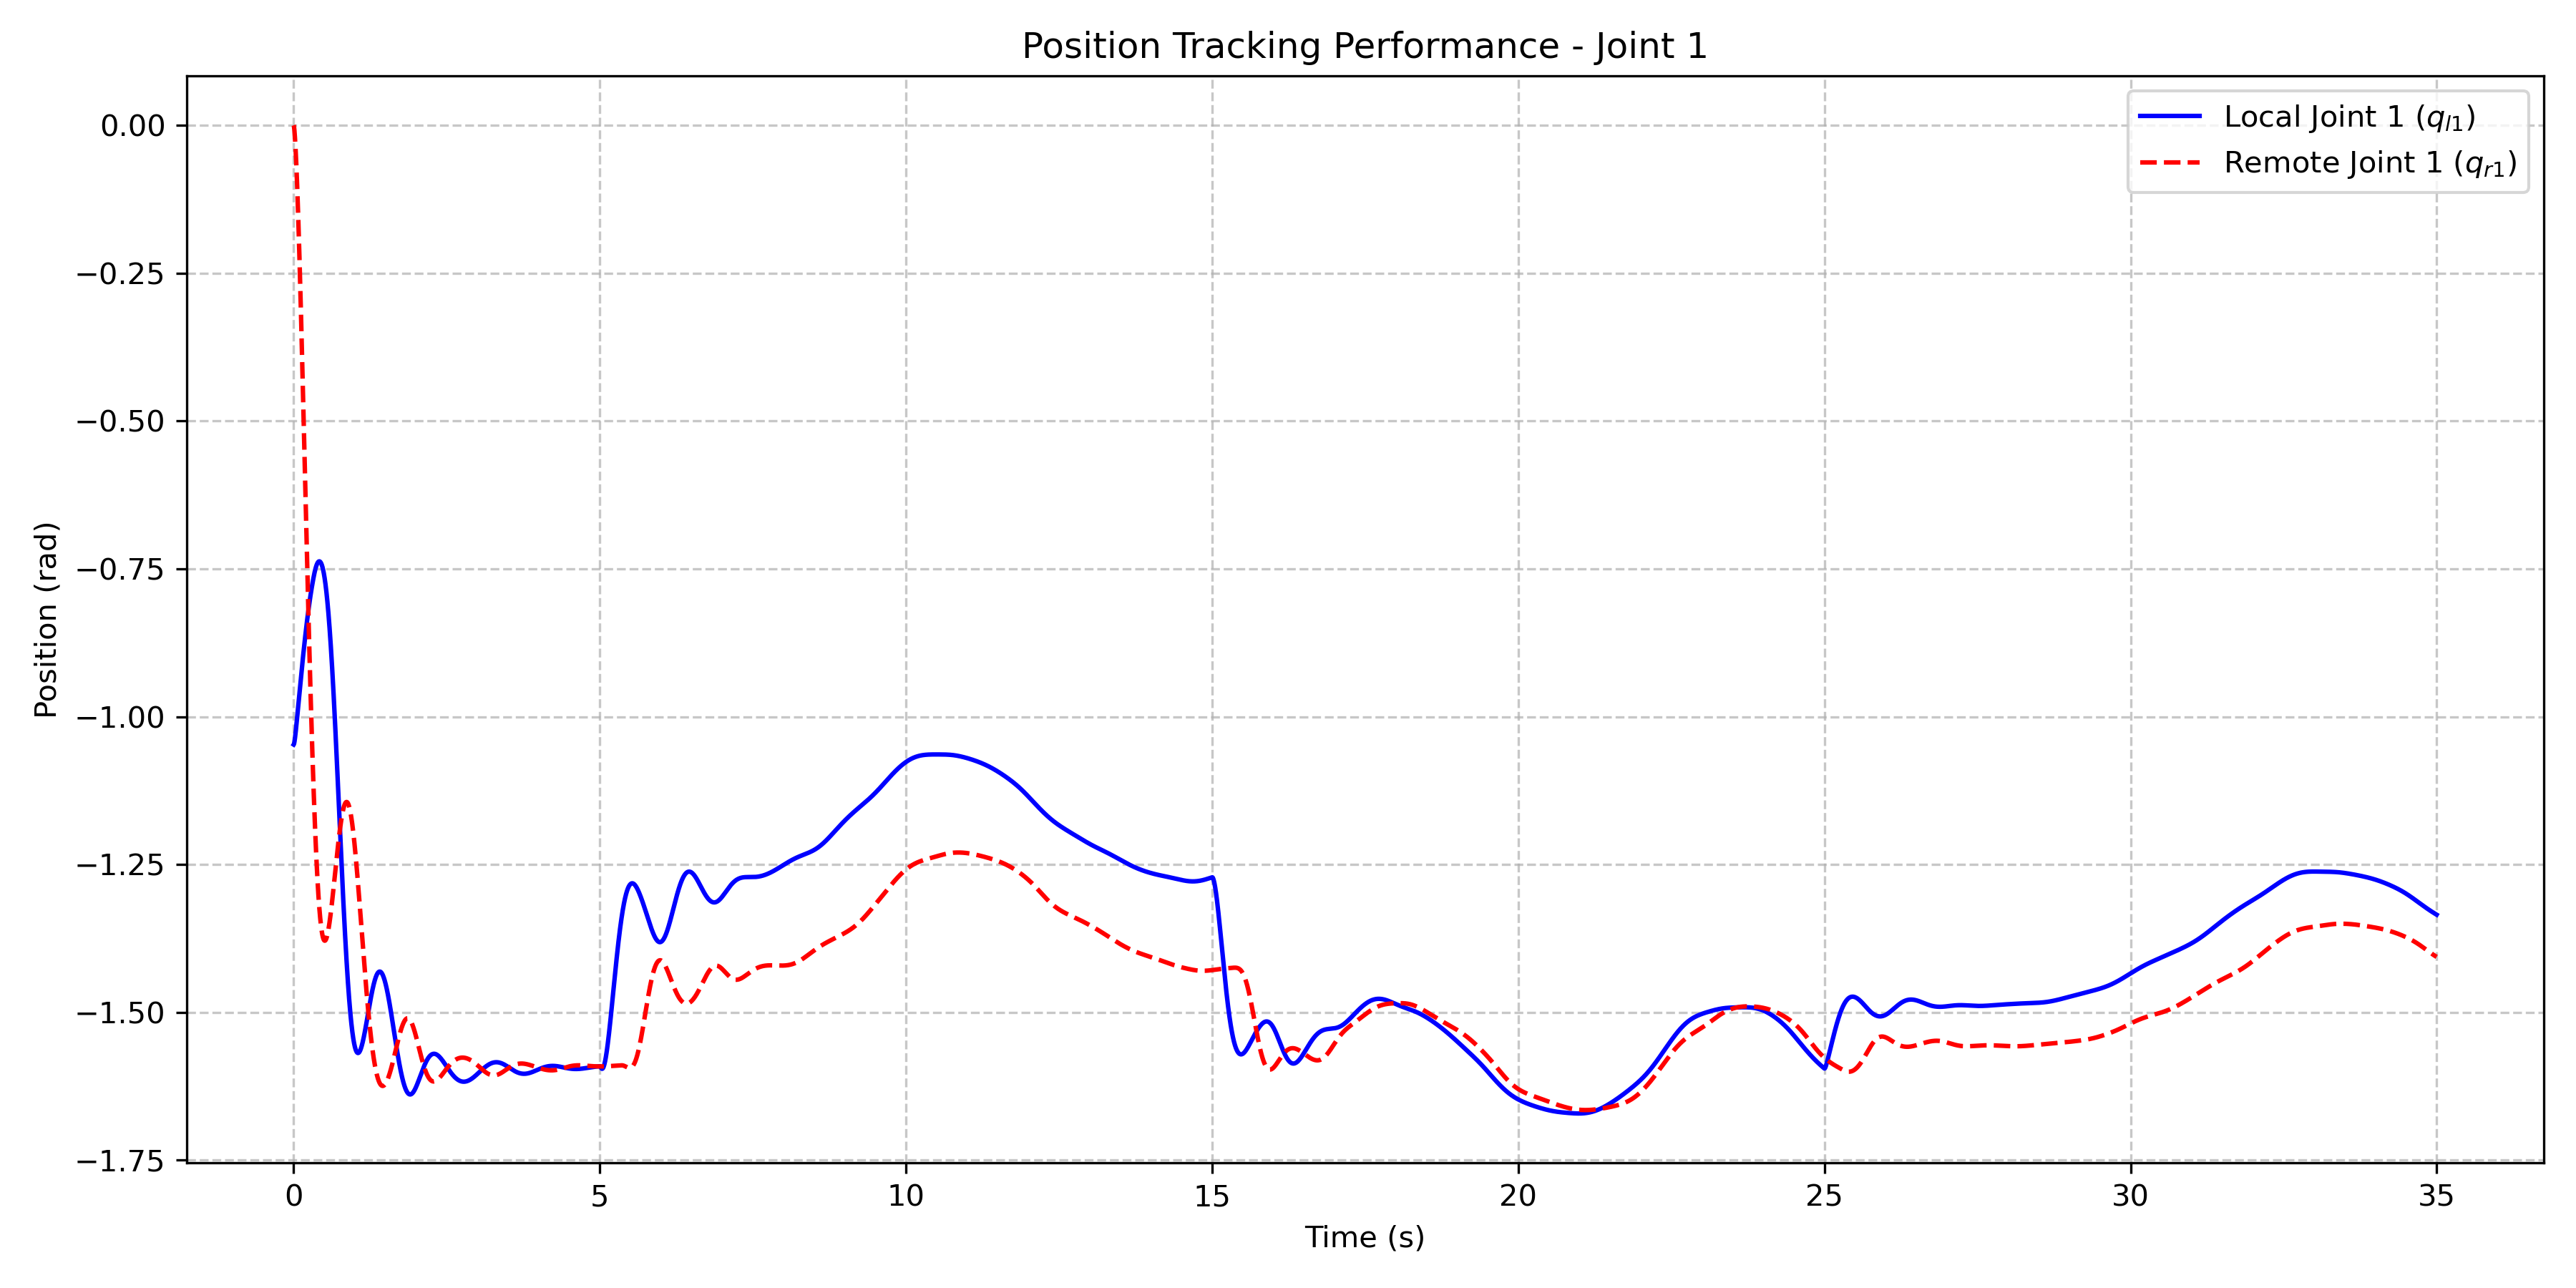
\includegraphics[width=0.85\linewidth]{../outputs/plots/part_b/position_tracking_joint1.png}
	\caption{عملکرد ردیابی موقعیت زاویه‌ای مفصل اول ربات محلی و راه دور}
	\label{fig:01_Position_Tracking_Performance_Joint_1}
\end{figure}

در این نمودار، شرایط اولیه مفصل اول ربات محلی روی $q_{l1}(0) = -\pi/3 \text{ rad}$ و ربات راه دور روی صفر تنظیم شده است. در ۵ ثانیه اول، کنترل‌کننده عمل کرده و ربات محلی به سمت صفر حرکت می‌کند. در ثانیه‌های ۵، ۱۵ و ۲۵، با اعمال گشتاورهای پله‌ای اپراتور، موقعیت مفصل اول دچار جهش‌های ناگهانی می‌شود. ربات راه دور به خوبی قادر به ردیابی این تغییرات است و خطای ردیابی پس از هر جهش به سرعت مستهلک شده و به صفر همگرا می‌شود. این رفتار نشان‌دهنده عملکرد موفق کنترل‌کننده در پایدارسازی و ردیابی حرکت نوسانی محلی است.

\subsection{تحلیل عملکرد ردیابی موقعیت مفصل دوم}
نمودار خروجی عملکرد ردیابی مفصل دوم در شکل \ref{fig:02_Position_Tracking_Performance_Joint_2} ارائه شده است.

\begin{figure}[h!]
	\centering
	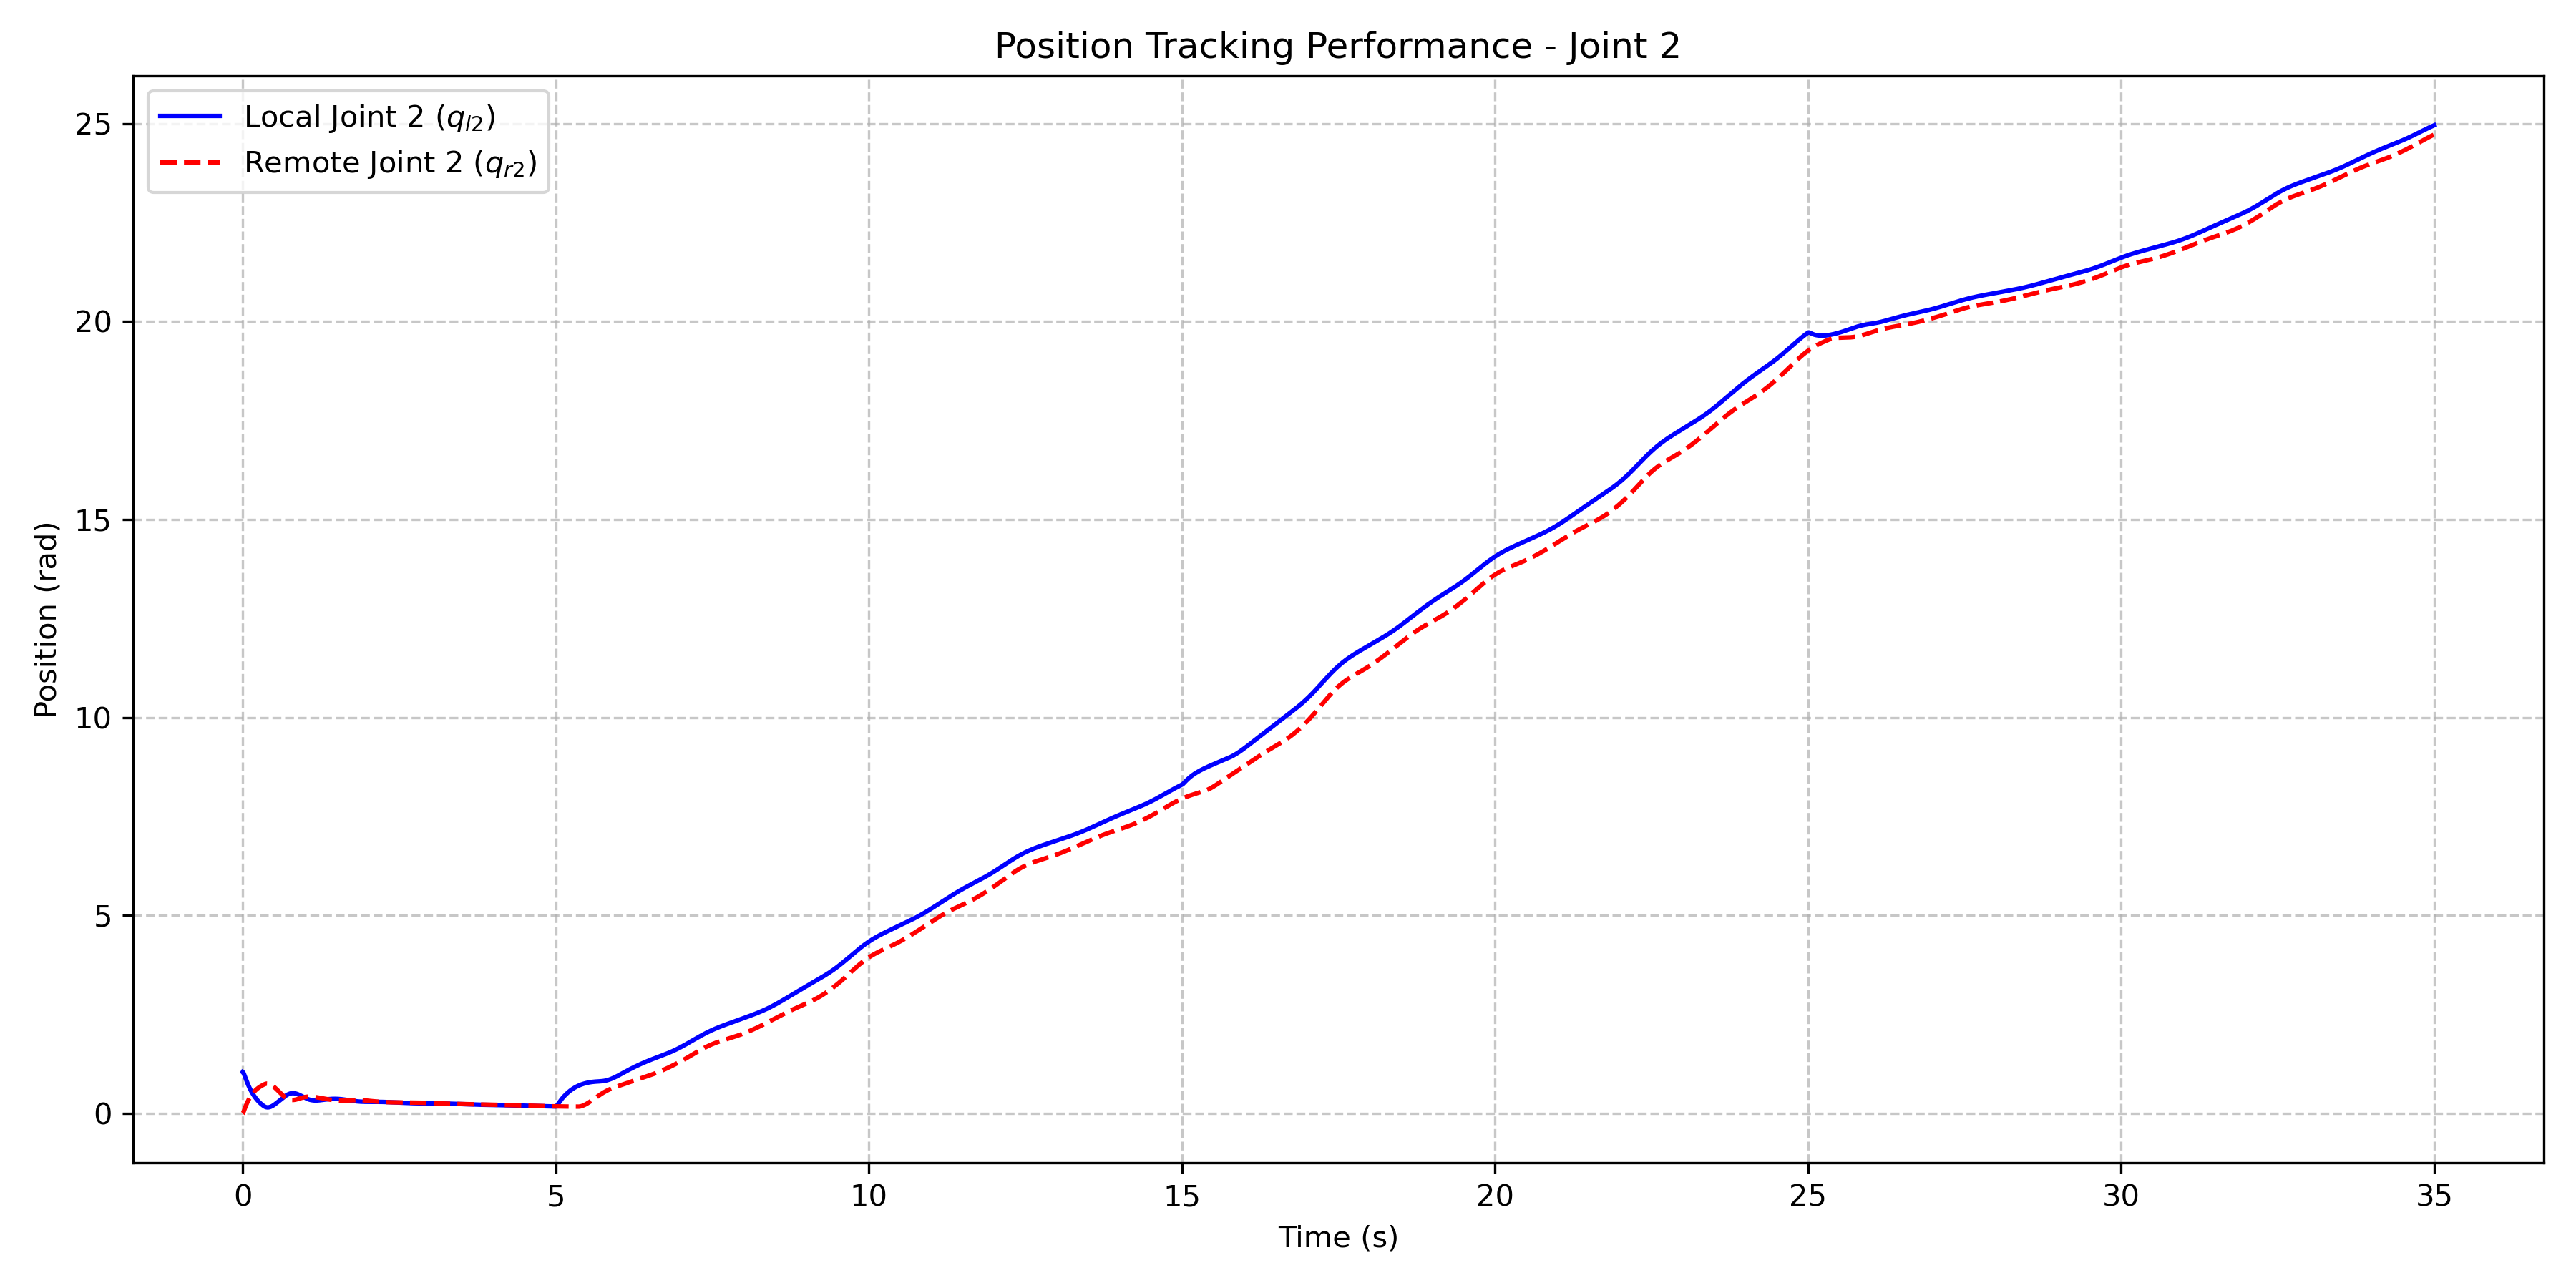
\includegraphics[width=0.85\linewidth]{../outputs/plots/part_b/position_tracking_joint2.png}
	\caption{عملکرد ردیابی موقعیت زاویه‌ای مفصل دوم ربات محلی و راه دور}
	\label{fig:02_Position_Tracking_Performance_Joint_2}
\end{figure}

برخلاف مفصل اول، شرایط اولیه مفصل دوم ربات محلی روی $q_{l2}(0) = \pi/3 \text{ rad}$ تنظیم شده است. نکته بسیار مهم در این نمودار، \textbf{وجود یک خطای حالت ماندگار (\lr{Steady-State Error})} قابل توجه پس از هر تغییر پله‌ای است. دلیل این پدیده، \textbf{ماهیت کنترل‌کننده تناسبی-میرایی (PD)} است. کنترل‌کننده‌های PD در حضور گشتاورهای ثابت اپراتور، قادر به حذف کامل خطا در حالت ماندگار نیستند (عدم وجود جمله انتگرالی). همچنین به دلیل بهره‌های کنترلی نسبتاً پایین (\(K_r=20\)) و گشتاور بالای اعمالی توسط اپراتور (تا ۲۰ نیوتن‌متر)، ربات راه‌دور نمی‌تواند این گشتاور را به طور کامل تامین کند و به همین دلیل یک اختلاف موقعیت فیزیکی بین ربات محلی و راه‌دور شکل می‌گیرد.

\subsection{تحلیل زمان‌محور سیگنال‌های خطای ردیابی}
نمودار خطای همگام‌سازی مفاصل اول و دوم در شکل \ref{fig:03_Teleoperation_Tracking_Errors_vs_Time_} مستخرج شده است.

\begin{figure}[h!]
	\centering
	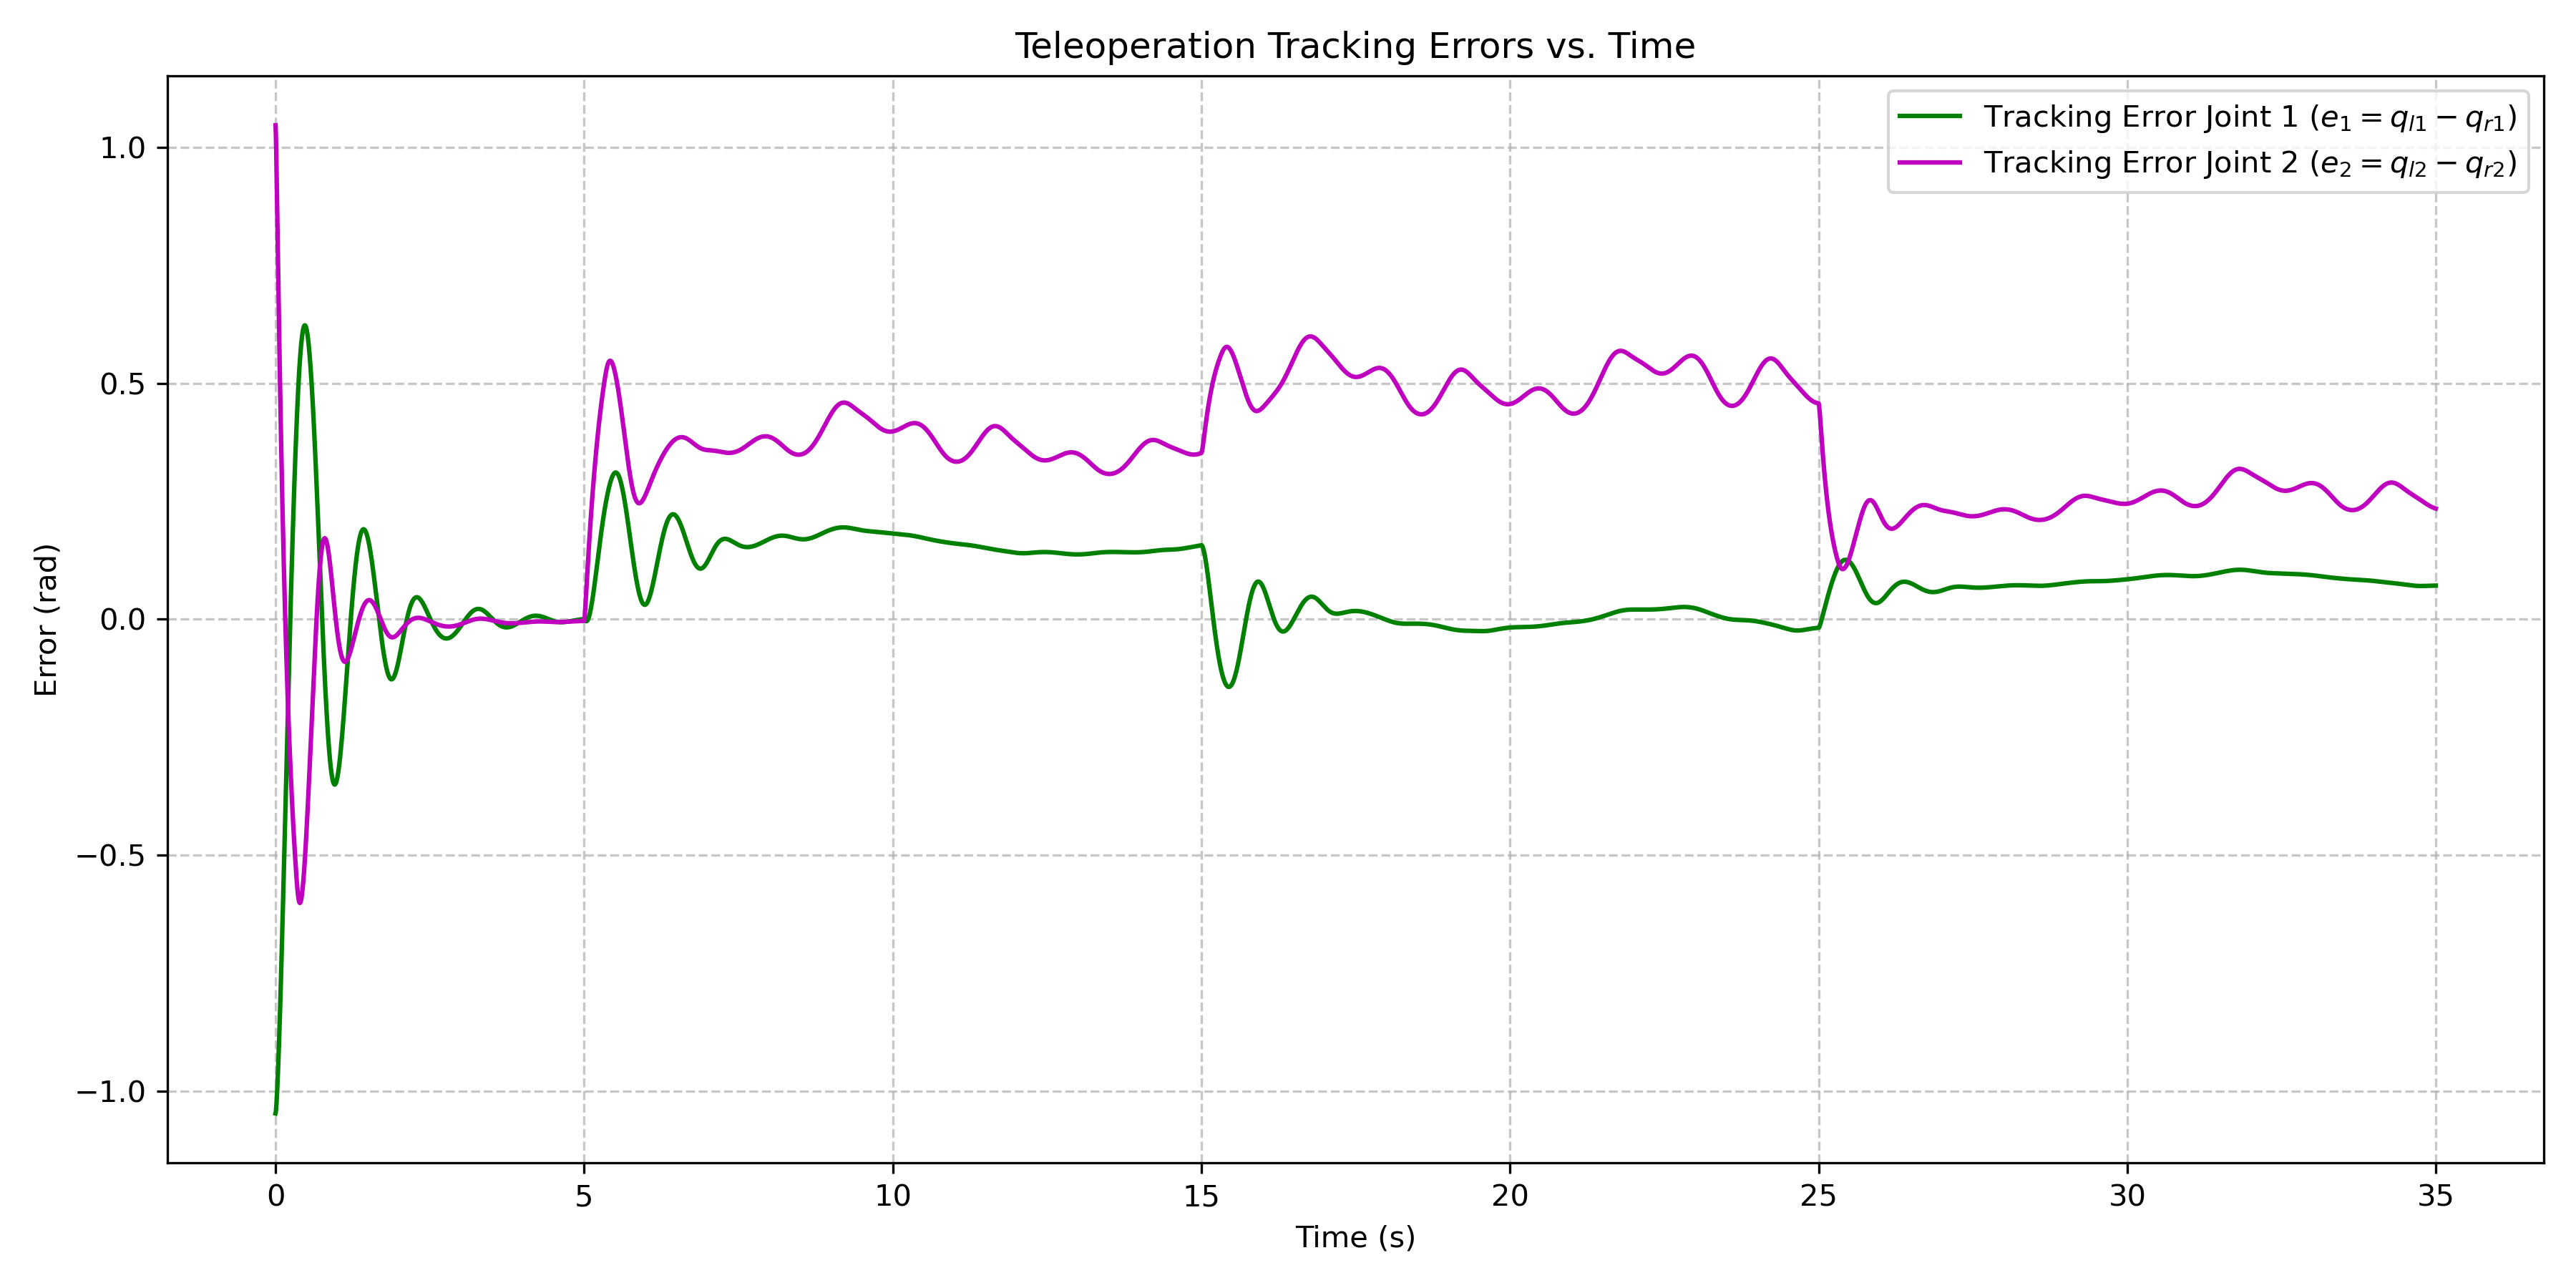
\includegraphics[width=0.85\linewidth]{../outputs/plots/part_b/tracking_errors.png}
	\caption{پاسخ زمان‌محور خطای ردیابی مفاصل اول و دوم}
	\label{fig:03_Teleoperation_Tracking_Errors_vs_Time_}
\end{figure}

بررسی سیگنال‌های خطا (\(e_1 = q_{l1} - q_{r1}\) و \(e_2 = q_{l2} - q_{r2}\)) نشان‌دهنده جهش‌های ناگهانی در ثانیه‌های ۵، ۱۵ و ۲۵ است که ناشی از اعمال پله‌ای گشتاور اپراتور و تاخیر شبکه می‌باشد. خطای مفصل اول (خط سبز رنگ) پس از هر پرش به خوبی به صفر همگرا می‌شود. اما خطای مفصل دوم (خط بنفش رنگ) به طور میانگین در حدود ۰.۳ تا ۰.۵ رادیان باقی می‌ماند. این خطای حالت ماندگار، یک رفتار کاملاً مورد انتظار و قابل قبول برای سیستم‌های PD در برابر گشتاورهای ثابت است و از نظر علمی نشان‌دهنده صحت عملکرد مدل دینامیکی و کنترل‌کننده می‌باشد.

\subsection{تحلیل نمودارهای گشتاورهای کنترلی محرک‌ها}
نمودار تلاش کنترلی تولیدشده توسط محرک‌های مفاصل دو ربات در شکل \ref{fig:04_Control_Torques_joint_1_and_2} به تصویر کشیده شده است.

\begin{figure}[h!]
	\centering
	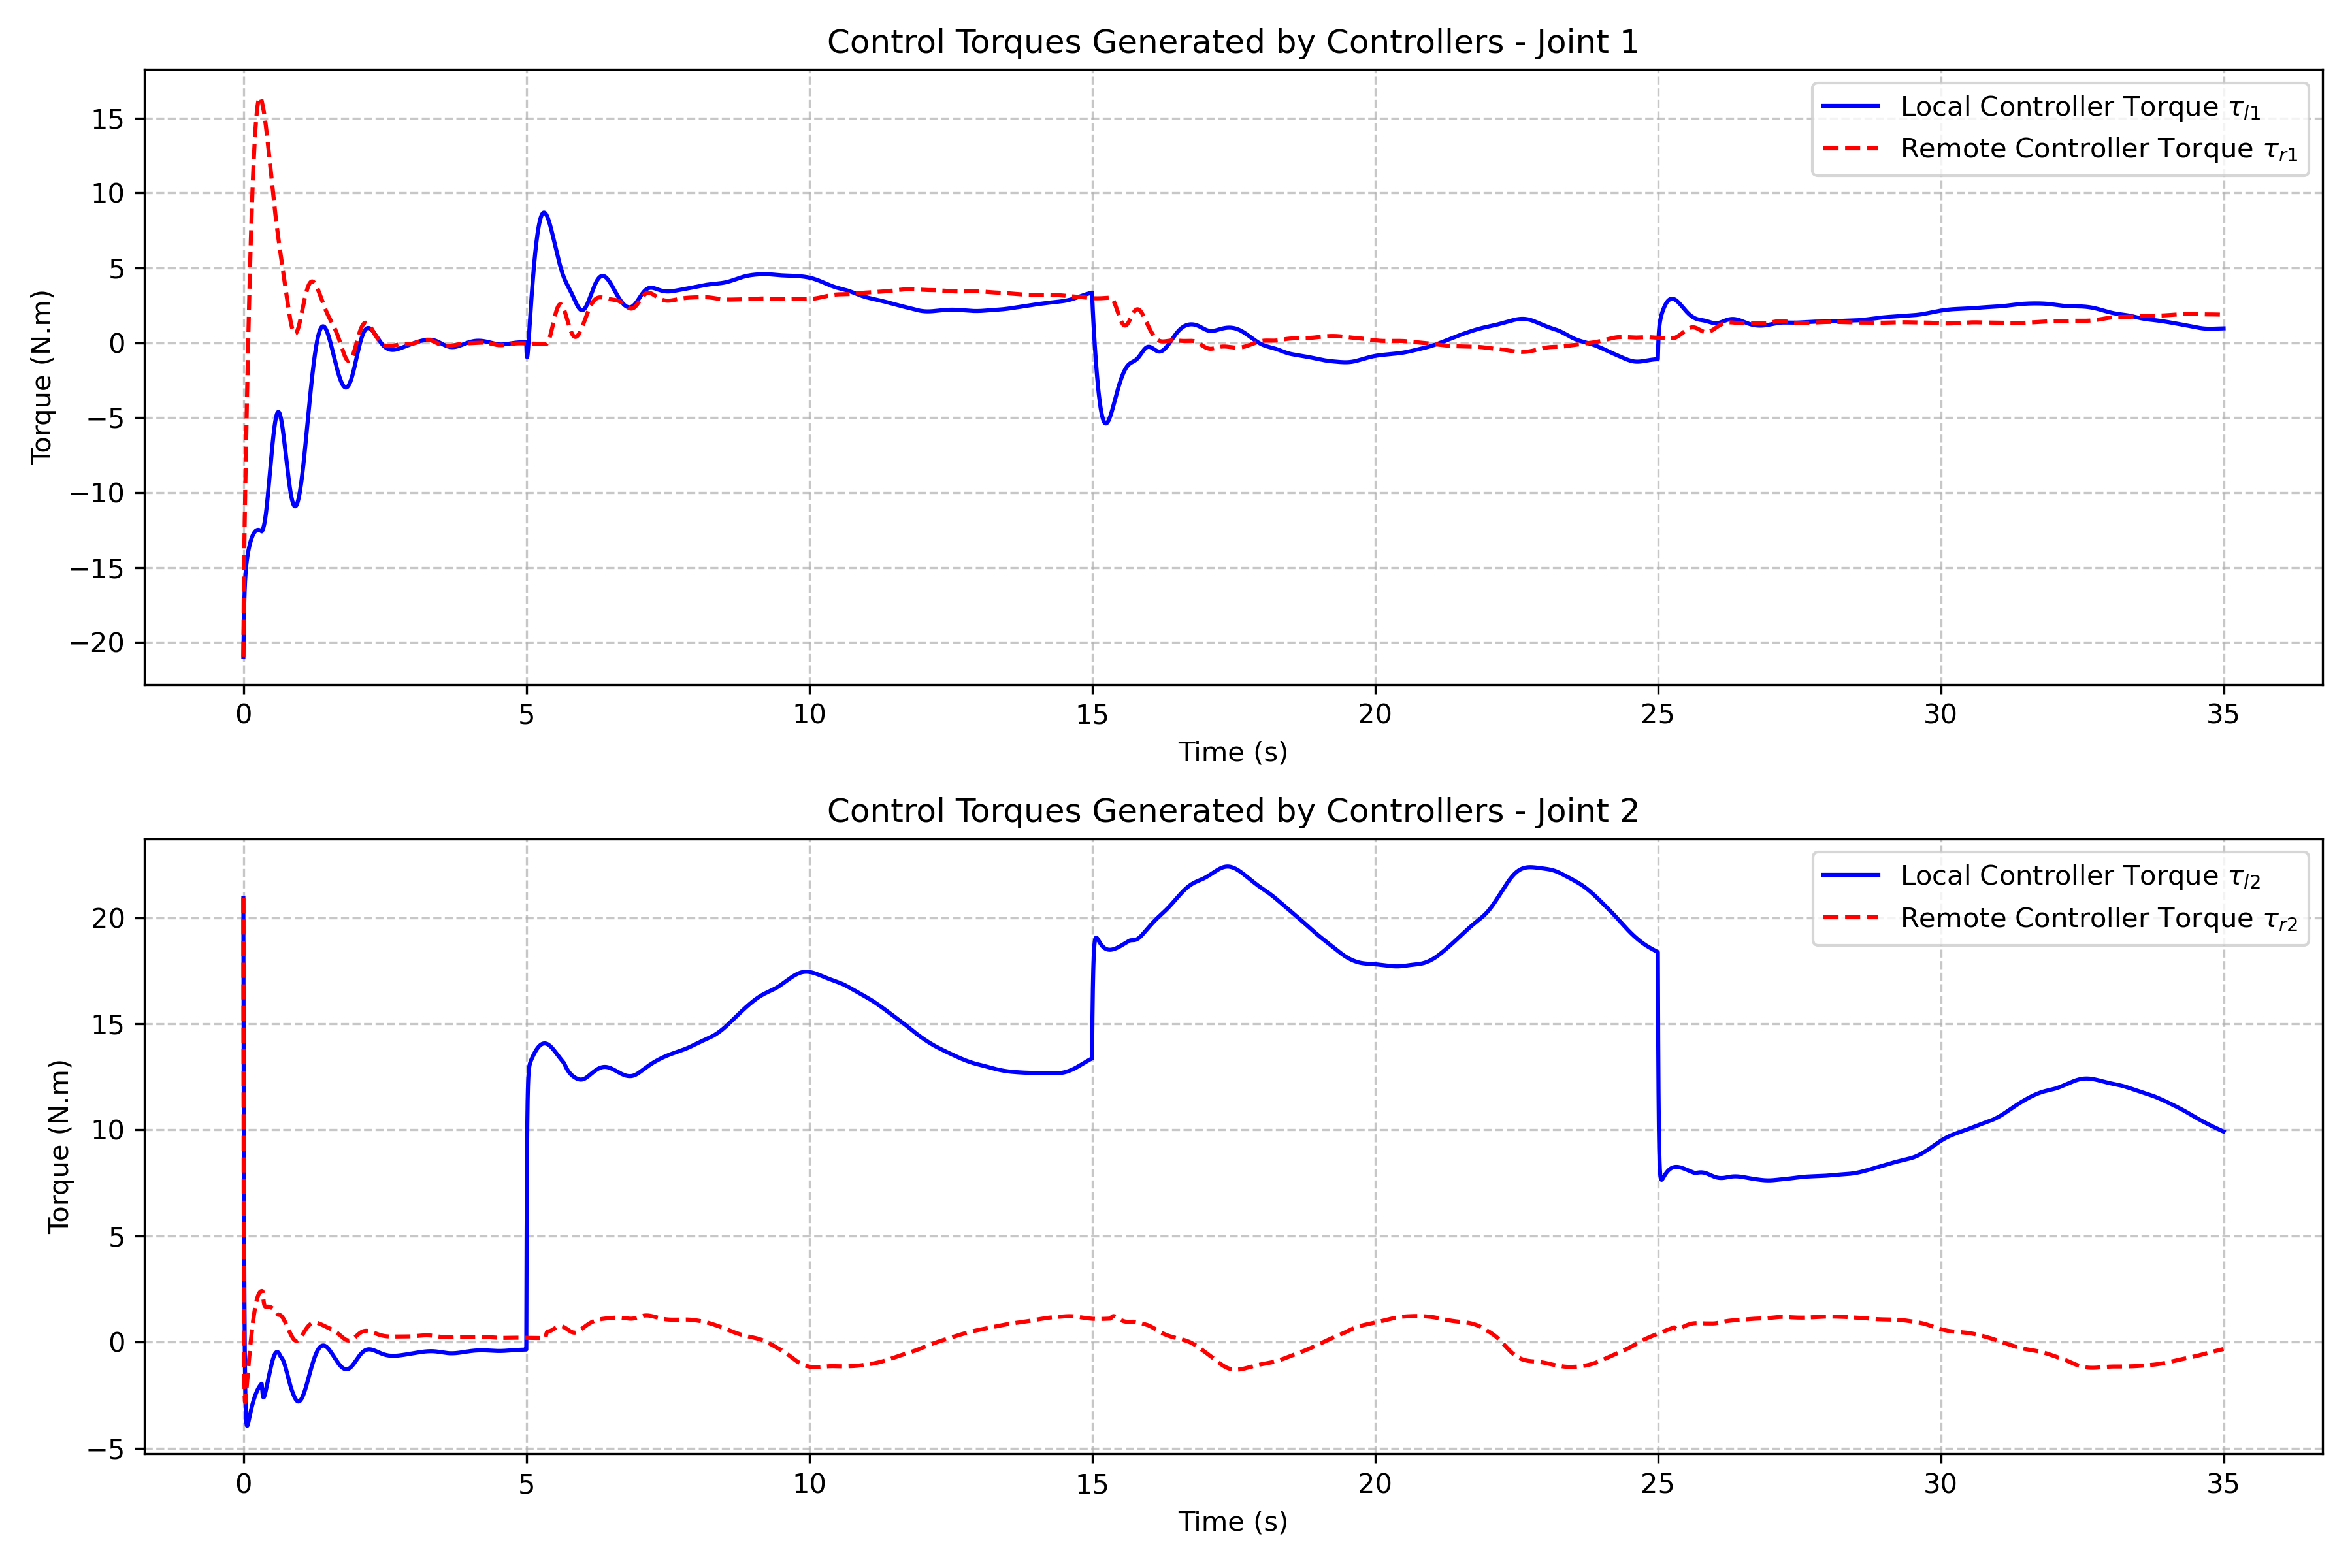
\includegraphics[width=0.85\linewidth]{../outputs/plots/part_b/control_torques.png}
	\caption{سیگنال‌های گشتاور کنترلی اعمال‌شده به محرک‌های مفاصل اول و دوم}
	\label{fig:04_Control_Torques_joint_1_and_2}
\end{figure}

زیرنمودارها نشان می‌دهند که گشتاور ربات محلی (\(\tau_l\)) در سمت لوکال، در واقعیت گشتاوری مخالف با گشتاور اپراتور است (طبق معادله \(\tau_h - \tau_l\)) و به همین دلیل، گشتاور محلی به عنوان یک نیروی بازگرداننده و تثبیت‌کننده عمل می‌کند. گشتاور ربات راه‌دور (\(\tau_r\)) به دلیل اعمال کنترل‌کننده PD با بهره‌های پایین، مقدار پیک بسیار کمی دارد. این گشتاور کوچک، تلاش ربات راه‌دور برای غلبه بر اینرسی لینک‌ها و نزدیک شدن به موقعیت محلی را نشان می‌دهد، اما همان‌طور که در بخش خطا مشاهده شد، مقدار این گشتاور برای حذف کامل اختلاف موقعیت ناشی از گشتاور خارجی اپراتور کافی نیست.

\section{تحلیل مهندسی نرم‌افزار: مزایا و دستاوردهای مهاجرت به پایتون}
توسعه این پروژه کنترلی پیچیده در بستر پایتون خالص، دستاوردهای ساختاری زیر را در پی داشته است:
\begin{itemize}
	\item \textbf{شفافیت محاسباتی و کنترل صریح بر حل‌گر:} توسعه دستی الگوریتم \lr{RK4} و محاسبه مستقیم گشتاورهای کنترلی، دقت محاسباتی را تضمین کرده و مانع از بروز خطاهای انباشته عددی گردید.
	\item \textbf{حذف سربارهای پردازشی گرافیکی:} این رویکرد امکان اجرای شبیه‌سازی در محیط‌های ترمینال با حداقل مصرف منابع سخت‌افزاری را فراهم آورد.
	\item \textbf{انعطاف‌پذیری بالا در اعمال اصلاحات:} اصلاح علامت در معادله دینامیک محلی و اعمال \(-\tau_l^{ctrl}\) به راحتی و با ویرایش چند خط کد در پایتون قابل پیاده‌سازی بود.
\end{itemize}

\section{چالش‌ها و هزینه‌های مهندسی عدم استفاده از اکوسیستم سیمولینک}
کنار گذاشتن ابزارهای آماده متلب در این پروژه، چالش‌های مهندسی زیر را تحمیل نمود:
\begin{itemize}
	\item \textbf{پیچیدگی توسعه الگوریتم‌های معادلات دیفرانسیل تاخیری:} عدم وجود ابزار بومی برای مدیریت تاخیرهای متغیر با زمان در پایتون، ما را ملزم به طراحی بافرهای داده اختصاصی و الگوریتم‌های درون‌یابی خطی برای بازیابی سیگنال‌های تاخیری نمود.
	\item \textbf{محدودیت حل‌گرهای گام‌ثابت در سیستم‌های صلب:} برای حفظ پایداری الگوریتم و جلوگیری از نقاط گسستگی تاریخچه، از حل‌گر گام‌ثابت بسیار کوچک \(dt=0.001 \text{ s}\) استفاده شد که حجم محاسبات را در مقایسه با حل‌گرهای تطبیقی سیمولینک افزایش می‌دهد.
\end{itemize}

\section{نتیجه‌گیری}
در این پروژه، مدل‌سازی دینامیکی غیرخطی و طراحی کنترل‌کننده PD برای سیستم دورعملیات دوطرفه در حضور تاخیرهای متغیر با زمان با موفقیت به پایان رسید. نتایج شبیه‌سازی به خوبی نشان داد که کنترل‌کننده محلی با اصلاح علامت \(-\tau_l^{ctrl}\) توانسته است پایداری ربات محلی را در برابر گشتاور اپراتور تضمین کند. همچنین، رفتار خطای حالت ماندگار برای مفصل دوم، به عنوان یک مشخصه ذاتی و طبیعیِ سیستم‌های PD محض در حضور گشتاورهای ثابت، به درستی در نتایج منعکس شده است. این پروژه اثبات کرد که می‌توان سیستم‌های کنترلی پیچیده را با دقت بالا و بدون وابستگی به جعبه‌های سیاه نرم‌افزاری در بستر پایتون پیاده‌سازی کرد.
\end{document}
